%%%%%%%%%%%%%%%%%%%%%%%%%
%% Header for standard beamer presentation
%%
%%  PresentationHeader.tex
%%
%%%%%%%%%%%%%%%%%%%%%%%%%

\documentclass[english,10pt]{beamer}

%%%%%%%%%%%%%%%%%%%%
%% Include general header where common packages are defined
%%%%%%%%%%%%%%%%%%%%

% general packages without options
\usepackage{amsmath,amssymb,bbm}




%%%%%%%%%%%%%%%%%%%%
%% Idem general commands
%%%%%%%%%%%%%%%%%%%%

%%% Commands

\newcommand{\noun}[1]{\textsc{#1}}


%% Math

% Operators
\DeclareMathOperator{\Cov}{Cov}
\DeclareMathOperator{\Var}{Var}
\DeclareMathOperator{\E}{\mathbb{E}}
\DeclareMathOperator{\Proba}{\mathbb{P}}

\newcommand{\Covb}[2]{\ensuremath{\Cov\!\left[#1,#2\right]}}
\newcommand{\Eb}[1]{\ensuremath{\E\!\left[#1\right]}}
\newcommand{\Pb}[1]{\ensuremath{\Proba\!\left[#1\right]}}
\newcommand{\Varb}[1]{\ensuremath{\Var\!\left[#1\right]}}

% norm
\newcommand{\norm}[1]{\| #1 \|}


% amsthm environments
\newtheorem{definition}{Definition}



%% graphics

% renew graphics command for relative path providment only ?
%\renewcommand{\includegraphics[]{}}






\usetheme{Warsaw}

\setbeamertemplate{footline}[text line]{}
\setbeamercolor{structure}{fg=purple!50!blue, bg=purple!50!blue}

\setbeamercovered{transparent}


% shortened command for a justified frame
\newcommand{\jframe}[2]{\frame{\frametitle{#1}\justify{#2}}}



%%%%%%%%%%%%%%%%%%%%%
%% Begin doc
%%%%%%%%%%%%%%%%%%%%%

\begin{document}



\title{Thesis Progress Meeting}


\author{J.~Raimbault$^{1,2}$}

\institute{$^{1}$G{\'e}ographie-cit{\'e}s (UMR 8504 CNRS)\\
$^{2}$LVMT (UMR-T 9403 IFSTTAR)}


\date{June 10th 2016}


%%%%%%%%%%%%%%%%%%%%%%%%%%%%%%%%
\begin{frame}
\titlepage
\end{frame}

%\begin{frame}
%\tableofcontents
%\end{frame}
%%%%%%%%%%%%%%%%%%%%%%%%%%%%%%%%



\section{Achieved Work}


%\item Gibrat-interaction Network Necessity [1.5w]\medskip
%\item Back on Memoire and ongoing projects [1w]\medskip
%\item Write proposal for China [0.5w]\medskip
%\item Cybergeo (conference May 26th) [1.5w]\medskip
%\item Finish side project (Transportation) [0.5w]


%NetworkNecessity	1,7
%Cybergeo	1,6
%Misc (AlgoSR, Scaling, Zipf, Gov, Tech, Chine, SFI prep)	0,5
%Spatial Stats	0,5
%Side (Transportation&Ecotox)	0,5
%Organisation/Workflow	0,3
%Seminar/Conference/Course	0,3
%General Bibliography	0,1



\jframe{Achieved Work (by projects)}{
\begin{itemize}
\item Cybergeo [1.6w] (ETA 1.5w)\medskip
\item Gibrat-interaction [1.7w] (ETA 1.5w)\medskip
\item Spatial Statistics [0.5w]\medskip
\item Misc (AlgoSR, Scaling, MetaZipf, Lutecia, Chine, SFI prep.) [0.5w]\medskip
\item Organisation/conference/biblio [0.7w]\medskip
\item Side projects (Transportation, Ecotoxicology) [0.5w] (ETA 0.5w)\medskip
\end{itemize}
}



\section{Network Necessity}


%
%\sframe{Network Necessity}{
%\textbf{Simple toy models to test theoretical assumption of network necessity}
%
%\medskip
%
%$\rightarrow$ Extended Gibrat model for population growth within a city system (simplified Favaro-Pumain model or projected Cottineau-1.y.z model) with interactions. \textit{Idea :} Test if physical Network (feedback of physical flows) allows a better fit.
%
%\medskip
%
%\textbf{Rq. :} a lot of confusion on Gibrat Model :
%\begin{enumerate}
%\item Under classical independence assumptions, $Law(P)$ is known at any $t$ whatever the distribution of growth rates : no need to simulate).
%\item Furthermore, various formulation are possible : independent realizations across cities of the same random process $P(t)$ with varying non-stationary parameters $\mu(t)$, with interdependence captured in recurrence relation between successive expectancies ; or multi-dimensional random process $(P_i(t))$ with covariance structure $\Covb{P_i}{P_j}$ estimated in time.
%\end{enumerate}
%
%}
%
%\sframe{Empirical Results}{
%\textit{Work on Pumain-INED French cities database.}
%\medskip
%\textbf{Growth Rates are more log-normal than normal ! } (simple likelihood tests) - in fact $\Delta \log P$ closer from levy fat-tail distribution.
%\medskip
%\textbf{Non-stationarity of correlations in time and space : }
%\smallskip
%\centering
%%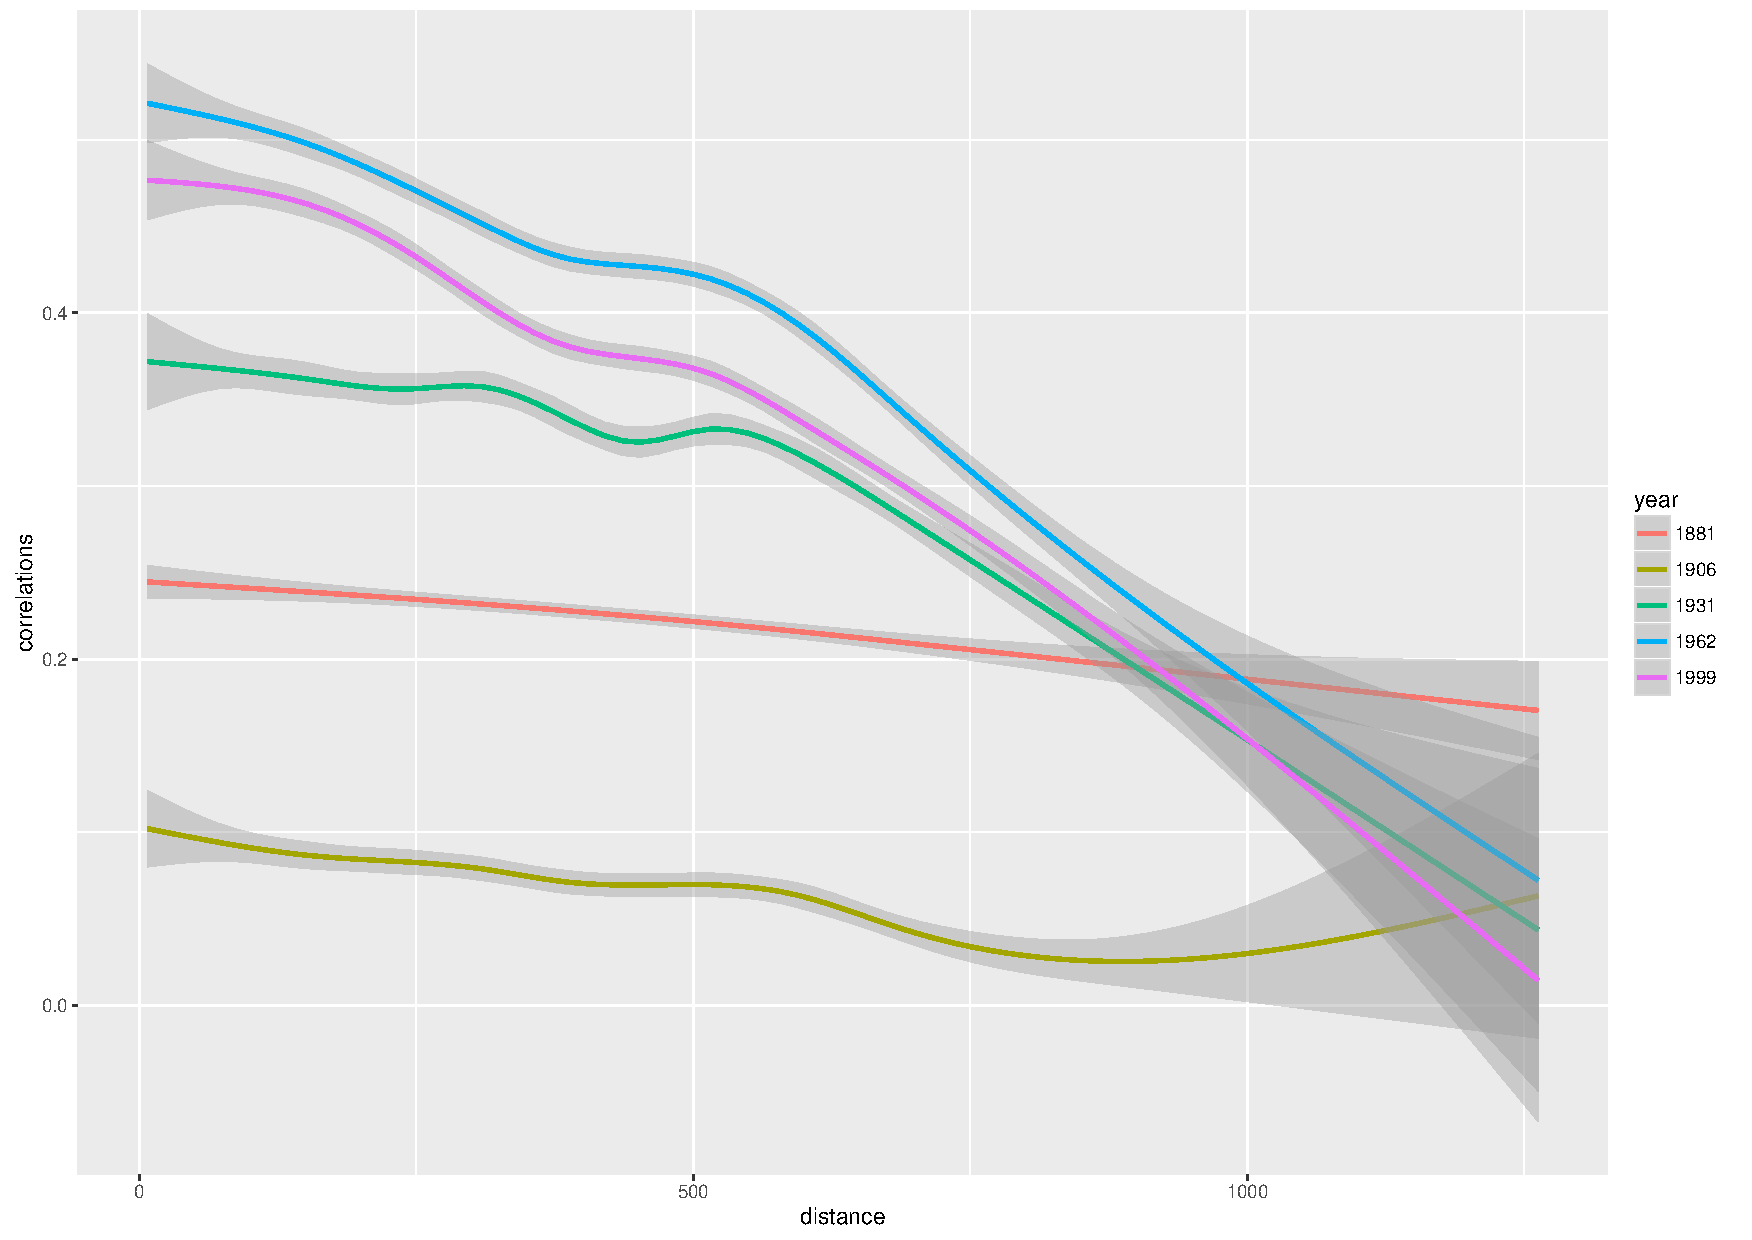
\includegraphics[width=0.6\textwidth]{figures/empirical_tsCorrelations}
%}

\sframe{Model Description}{

$\rightarrow$ Rationale : extend an interaction model for system of cities by including physical network, to investigate its influence on system dynamics

\medskip

$\rightarrow$ Work under Gibrat independence assumptions, i.e. $\Covb{P_i(t)}{P_j(t)}=0$. If $\vec{P}(t+1)=\mathbf{R}\cdot \vec{P}(t)$ where $\mathbf{R}$ is also independent, then $\Eb{\vec{P}(t+1)}=\mathbf{R}\cdot\Eb{\vec{P}}(t)$. Expectancies only for now (higher moments computable similarly)

\medskip

$\rightarrow$ With $\vec{\mu}(t)=\Eb{\vec{P}(t)}$, we generalize this approach by taking $\vec{\mu}(t+1)=f(\vec{\mu}(t))$

\medskip

$\rightarrow$ In our case, $f(\vec{\mu}) = r_0\cdot \mathbf{Id}\cdot \vec{\mu} + \mathbf{G}\cdot \mathbf{1} + \mathbf{N}\cdot $ with 
\begin{itemize}
\item $G_{ij} = w_G\cdot \frac{V_{ij}}{<V_{ij}>}$ and $V_{ij} = \left(\frac{\mu_i\mu_j}{\sum{\mu_k}^2}\right)^{\gamma_G} \exp{(-d_{ij}/d_G)}$
\item $N_{i} = w_N \cdot \sum_{kl} \left(\frac{\mu_k\mu_l}{\sum\mu}\right)^{\gamma_N}\exp{(-d_{kl,i})/d_N}$ where $d_{kl,i}$ is distance to shortest path between $k,l$ computed with slope impedance ($Z=\left(1+\alpha/\alpha_0\right)^{n_0}$ with $\alpha_0\simeq 3$)
\end{itemize}



%Interaction model with $\Eb{\vec{P} (t+1)}= (r_0\cdot \mathbf{Id}+\mathbf{R})\Eb{\vec{P}(t)}$, specified with gravity interactions $\left(\mathbf{R}[\cdot]\right)_{ij} = \frac{1}{V_0}\cdot\left(\frac{\Eb{P_j}\Eb{P_i}}{P^2}\right)^{\gamma}\cdot \exp{\left(-\frac{d_ij}{d_0}\right)}$ (note : taking $\gamma=1$ yields linear formulation).

%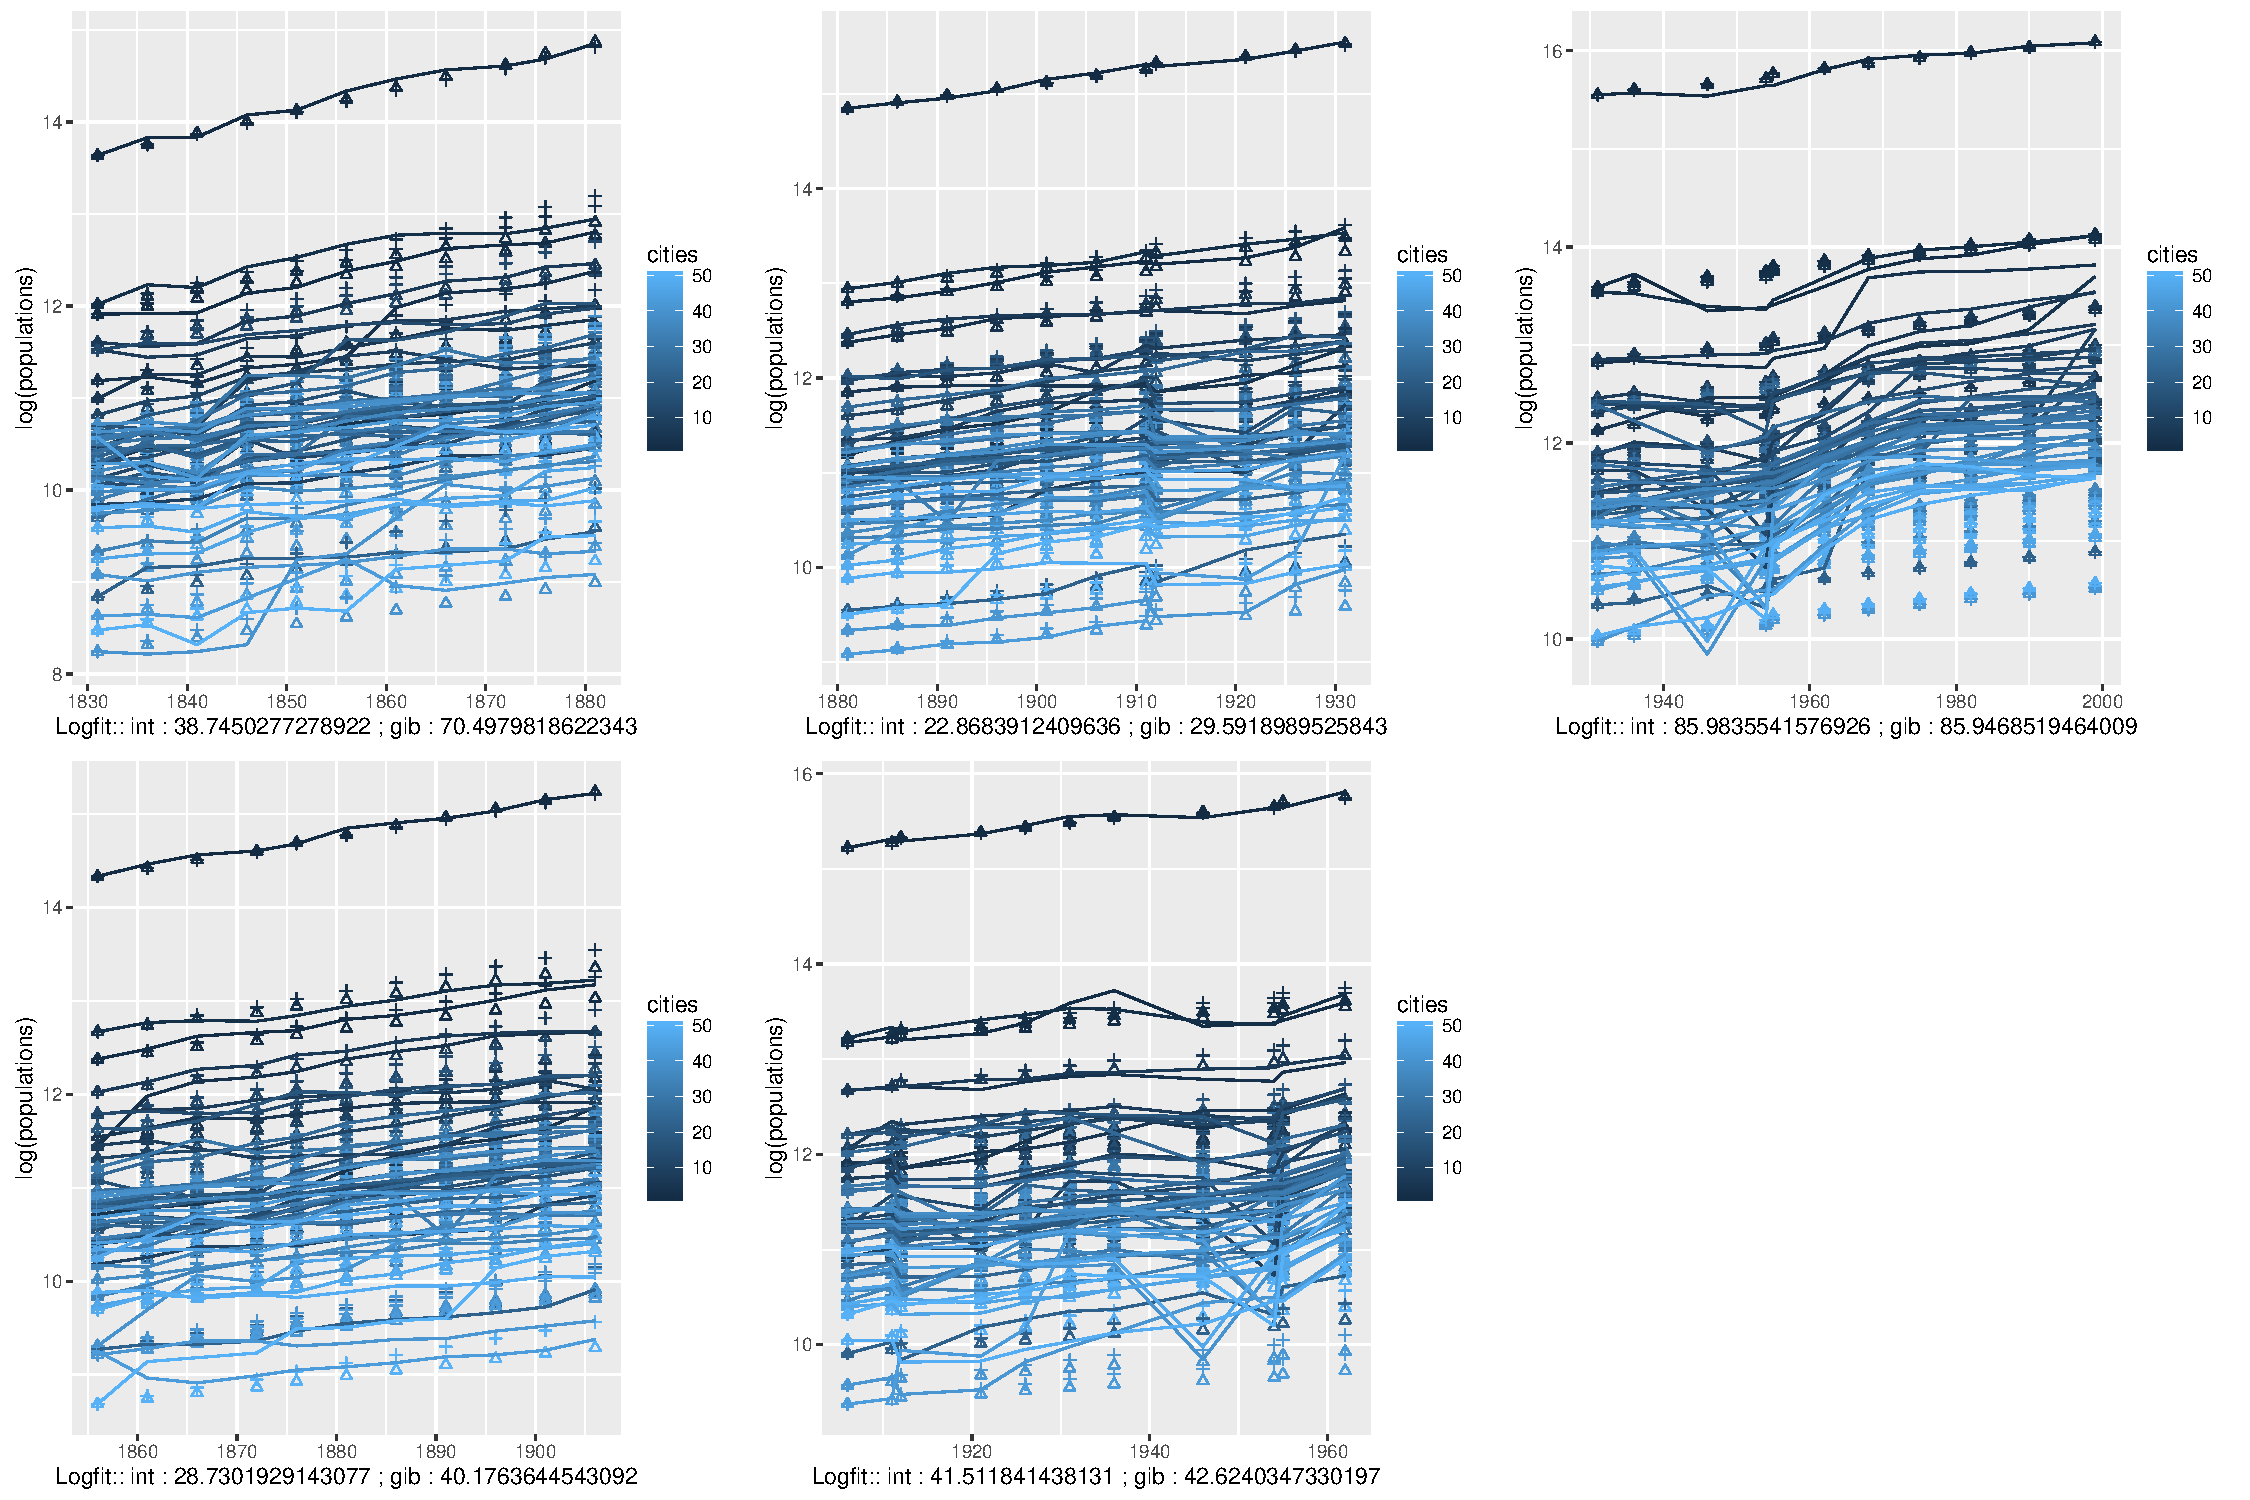
\includegraphics[width=0.8\textwidth]{figures/fit_intgib}
}

%
%\sframe{Spatialization}{
%
%}


\sframe{Exploration : Gravity Only}{
\textit{logmse : log of mean square error on populations}

\medskip

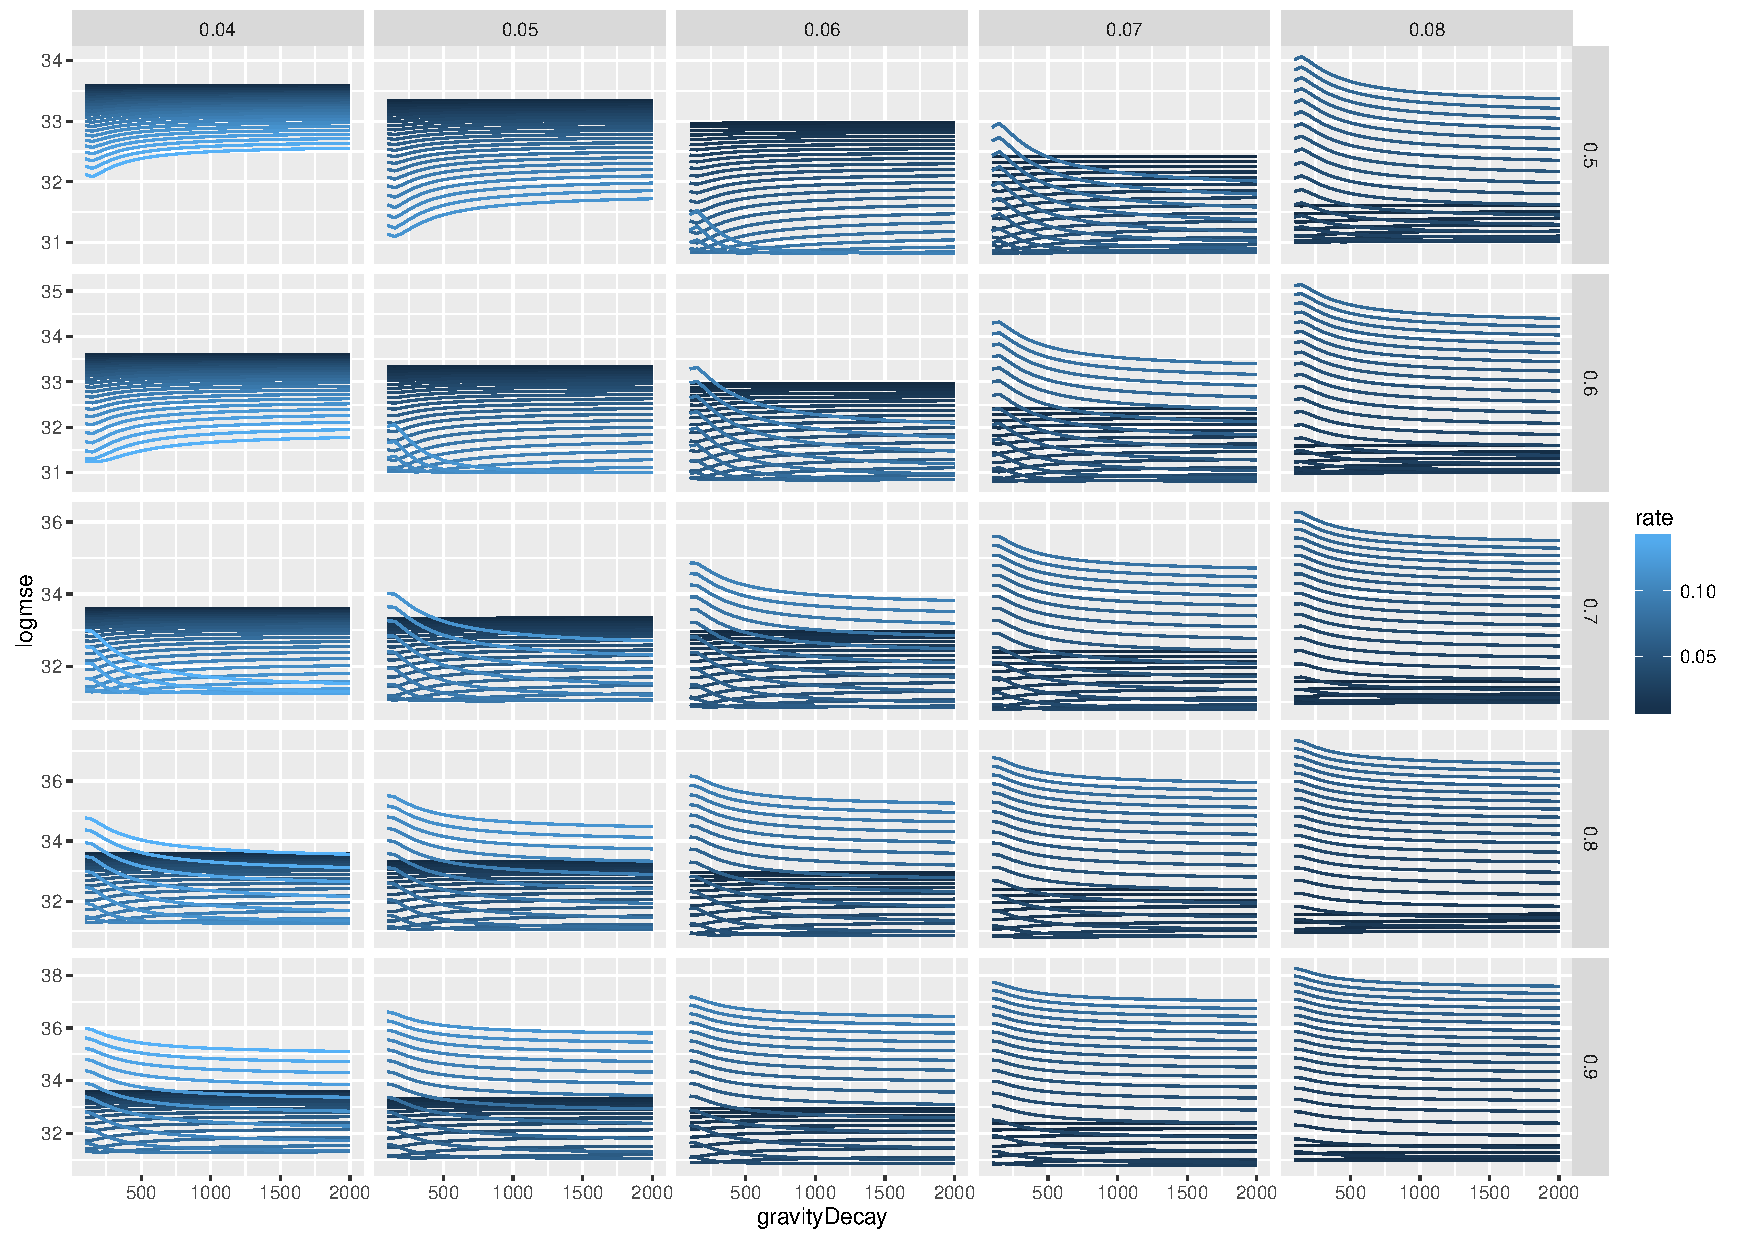
\includegraphics[width=0.55\textwidth]{figures/logmse-gravityDecay_facetgrowthRate-gravityGamma}
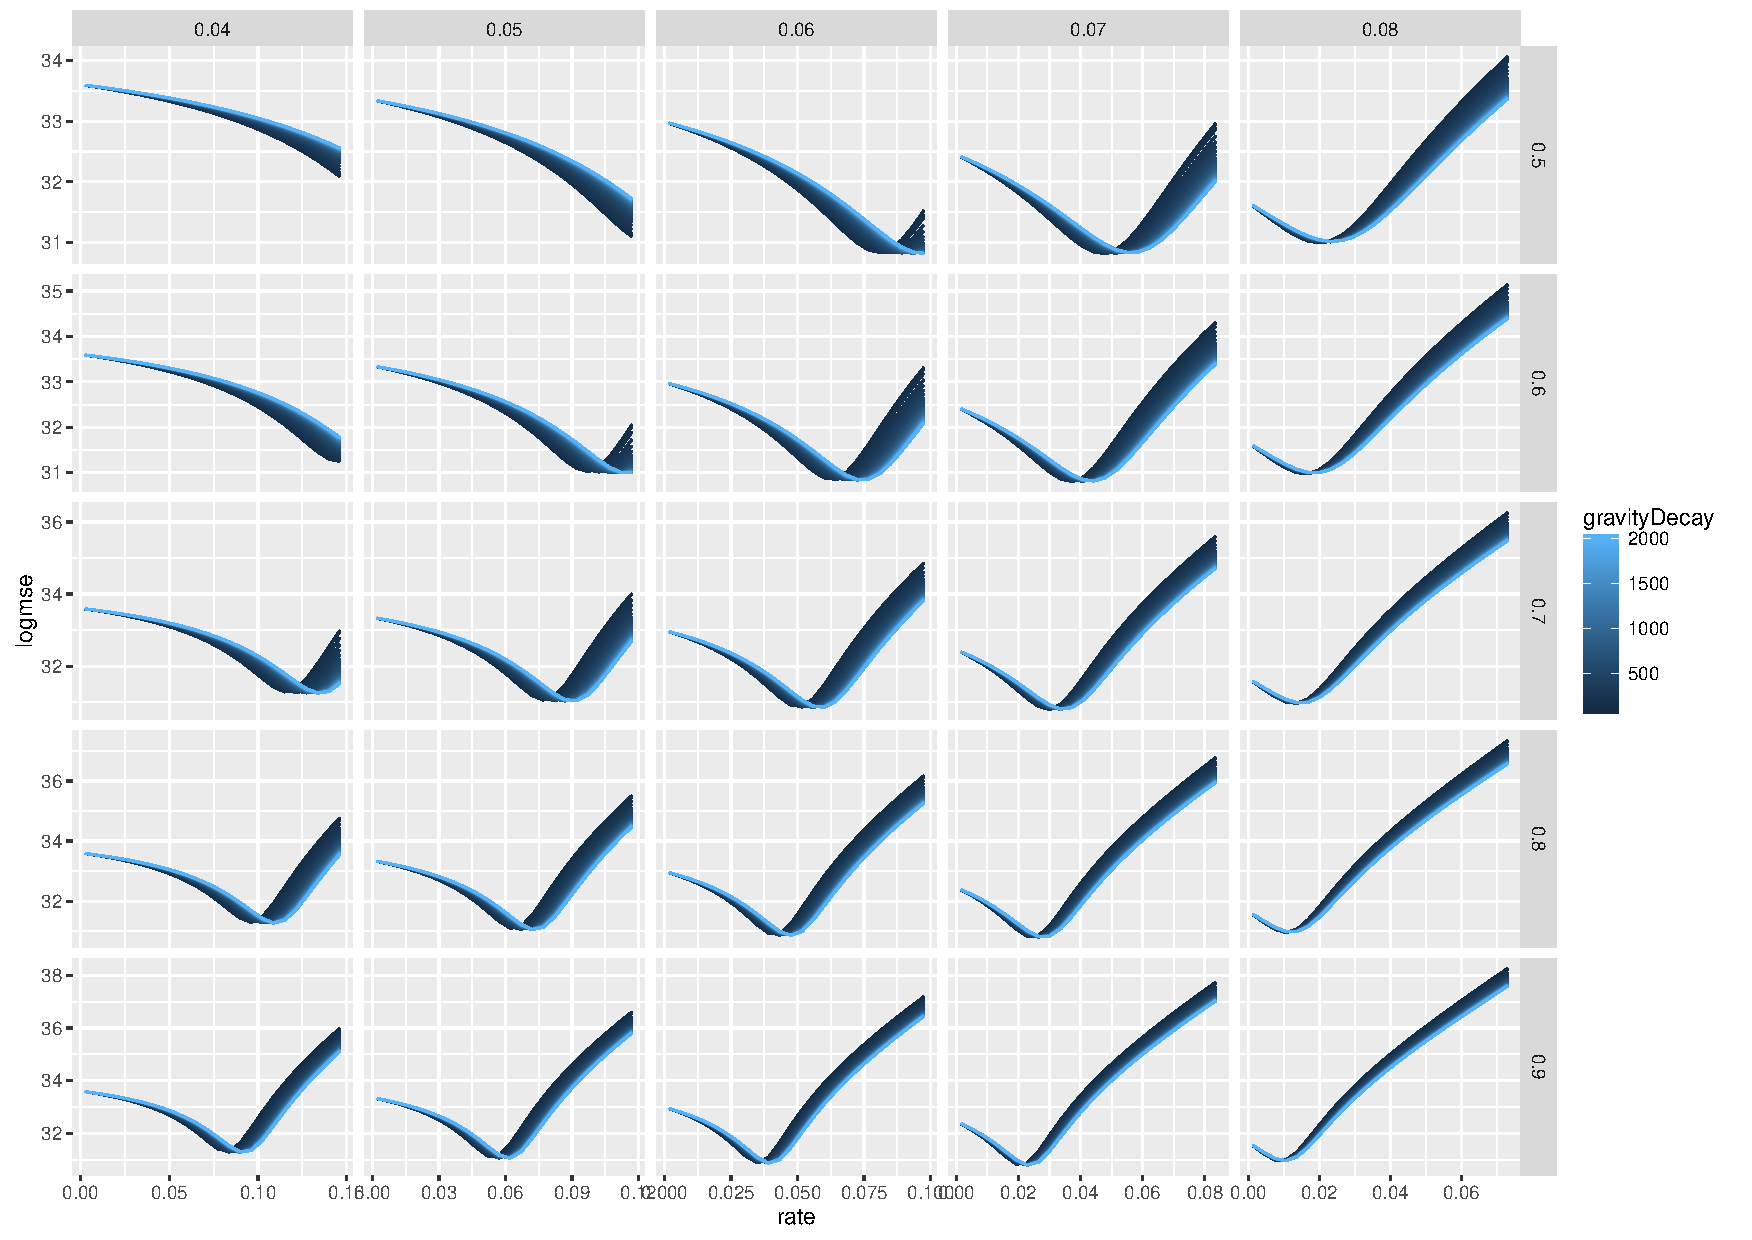
\includegraphics[width=0.55\textwidth]{figures/logmse-rate_facetgrowthRate-gravityGamma}

}

\sframe{Exploration : Gravity Only}{
\textit{mselog : mean square error on log of populations}

\medskip

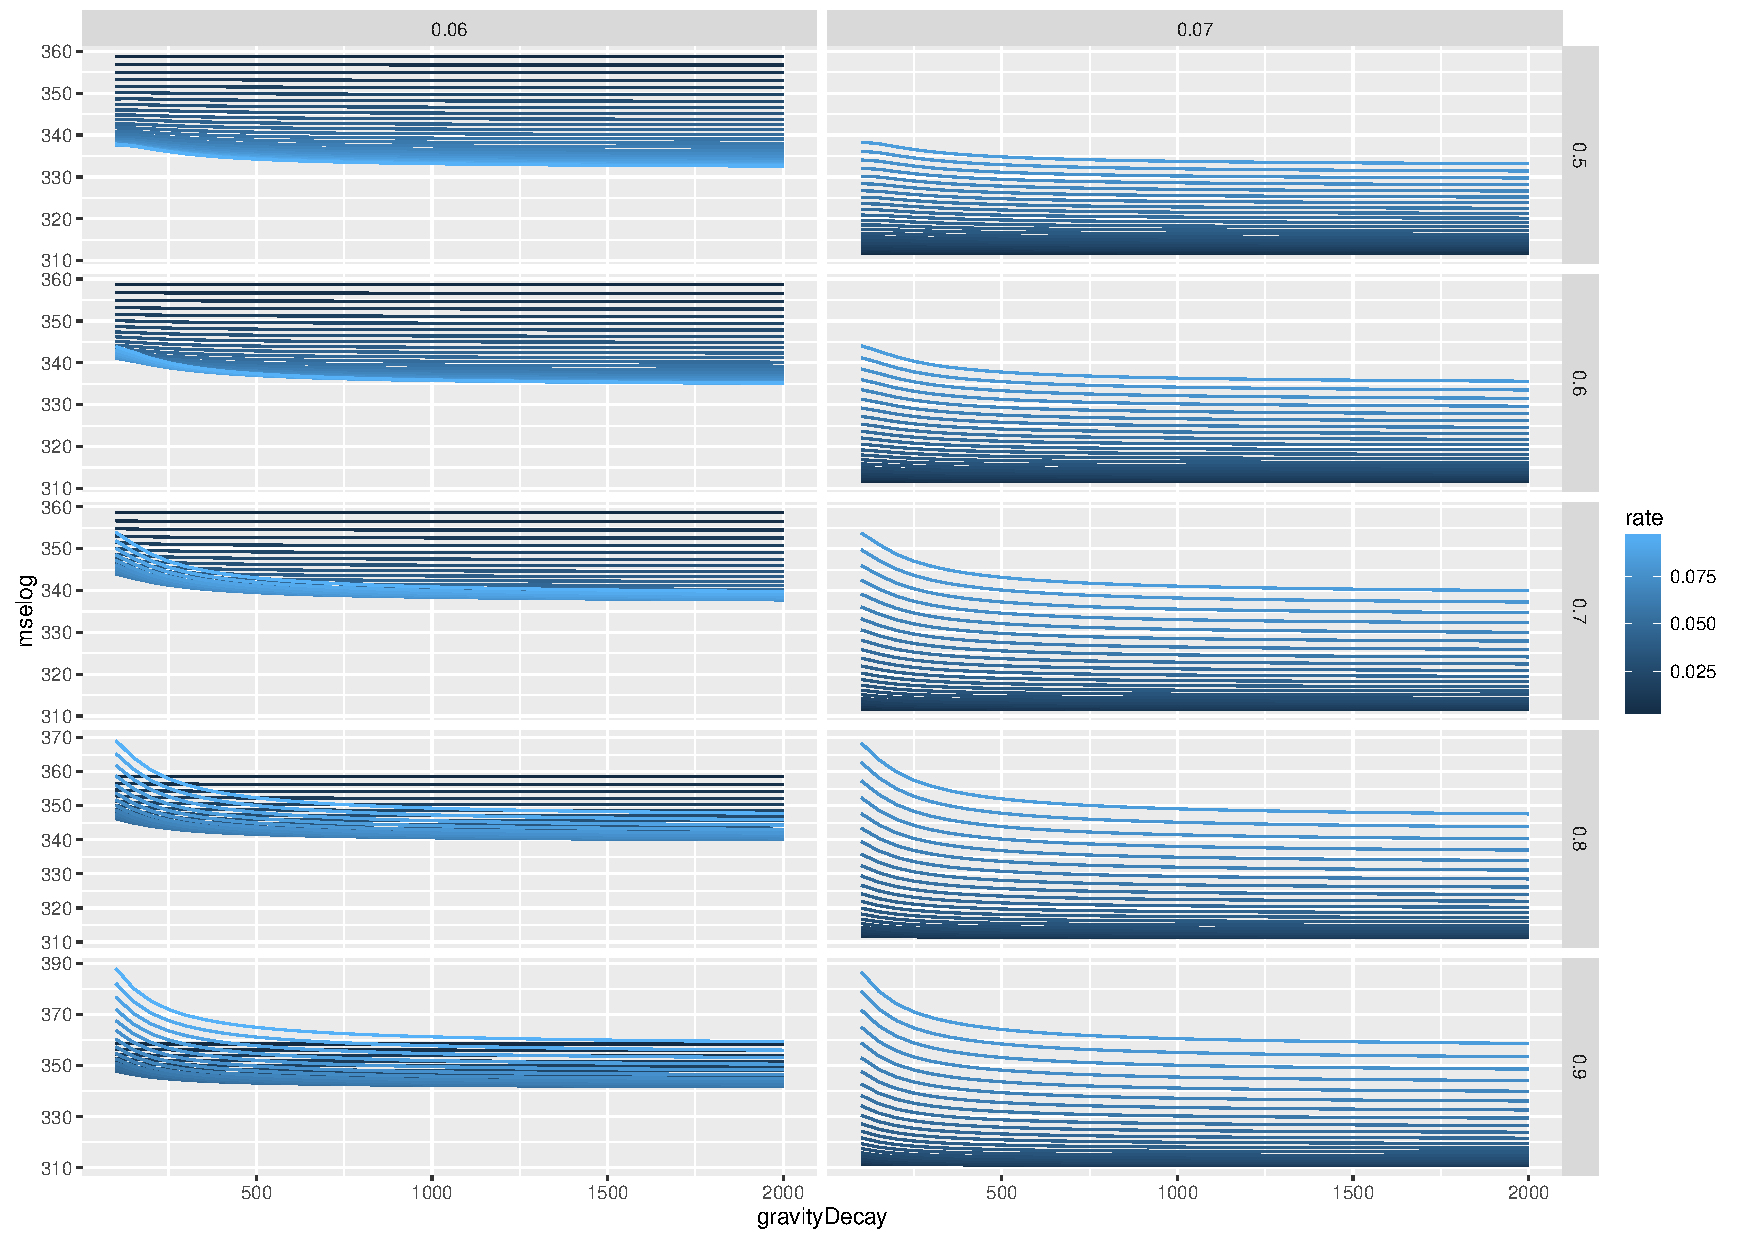
\includegraphics[width=0.55\textwidth]{figures/mselog-gravityDecay_facetgrowthRate-gravityGamma}
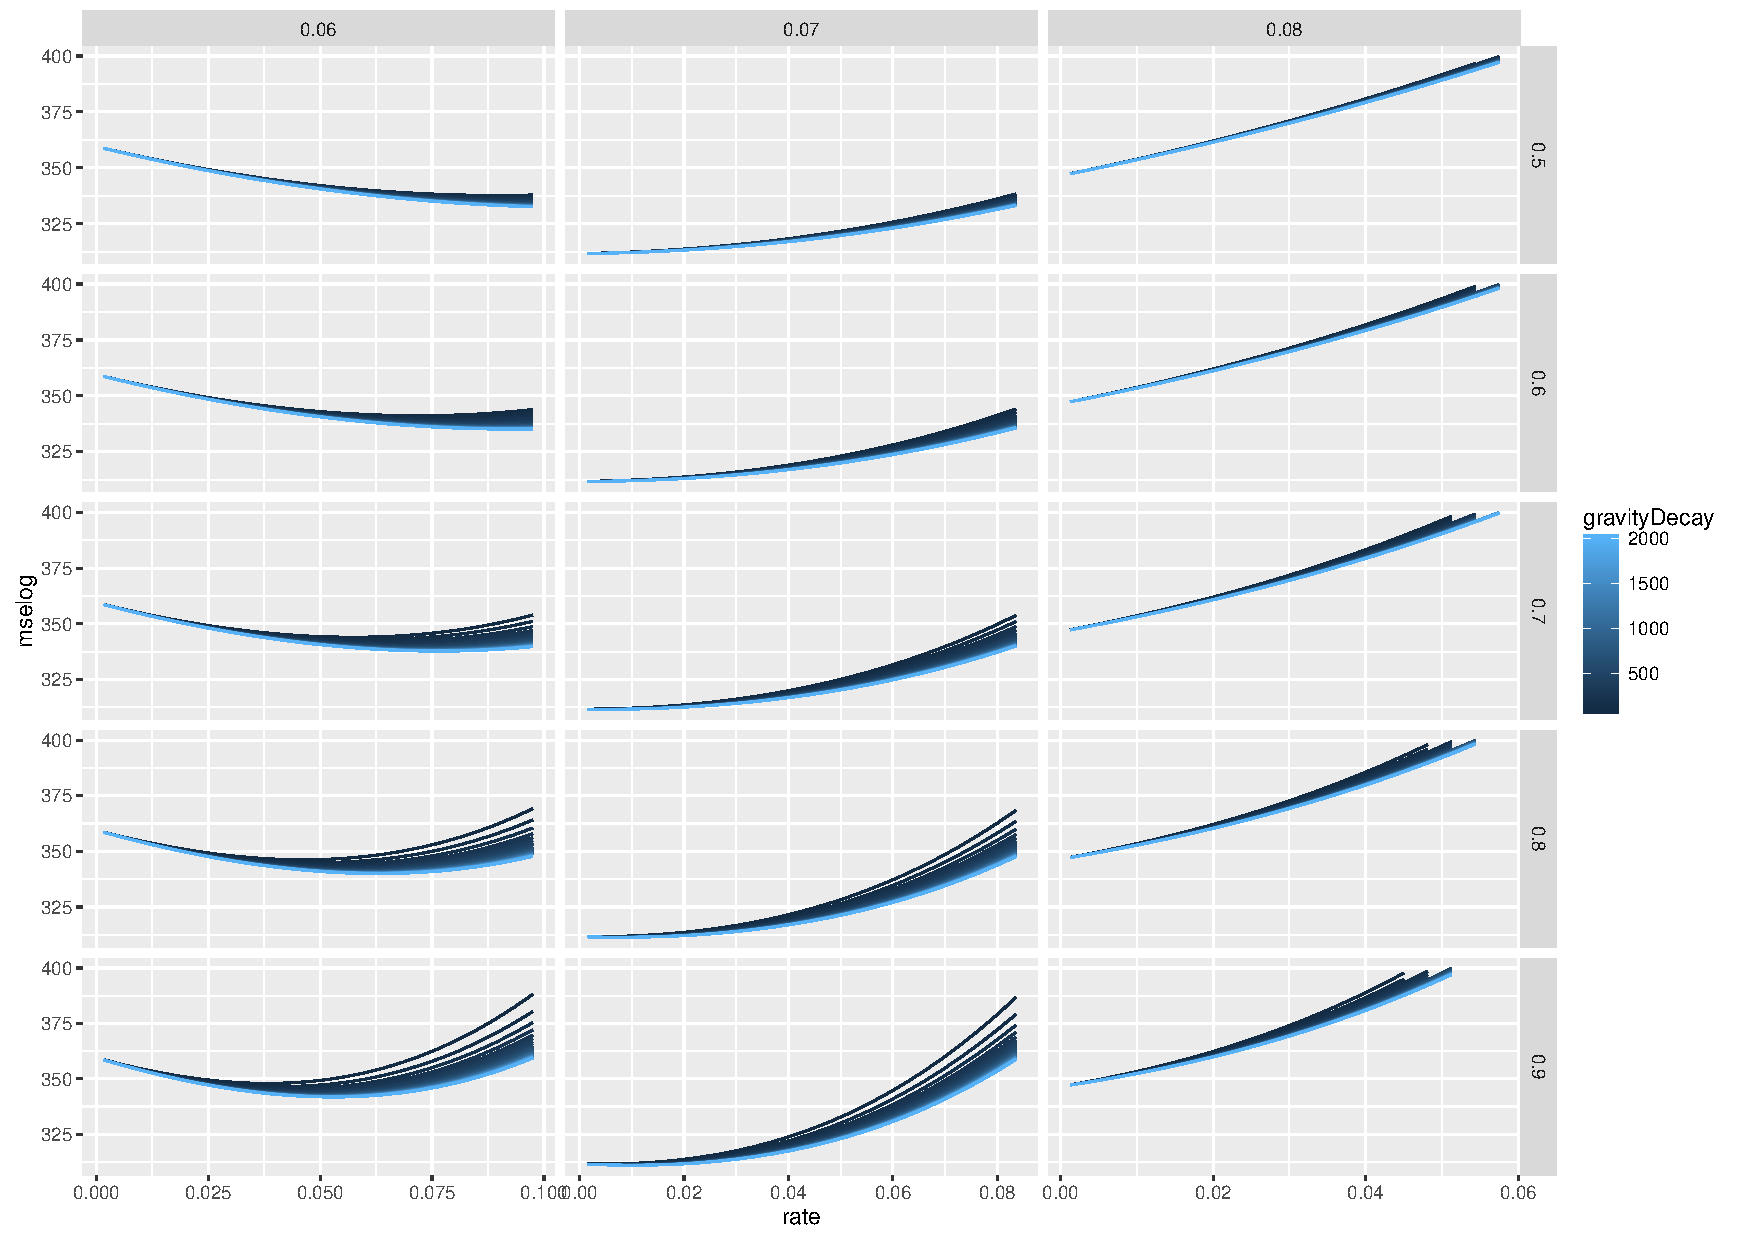
\includegraphics[width=0.55\textwidth]{figures/mselog-rate_facetgrowthRate-gravityGamma_ZOOM}

}




\sframe{Exploration}{
\textit{Feedback Only}

\medskip

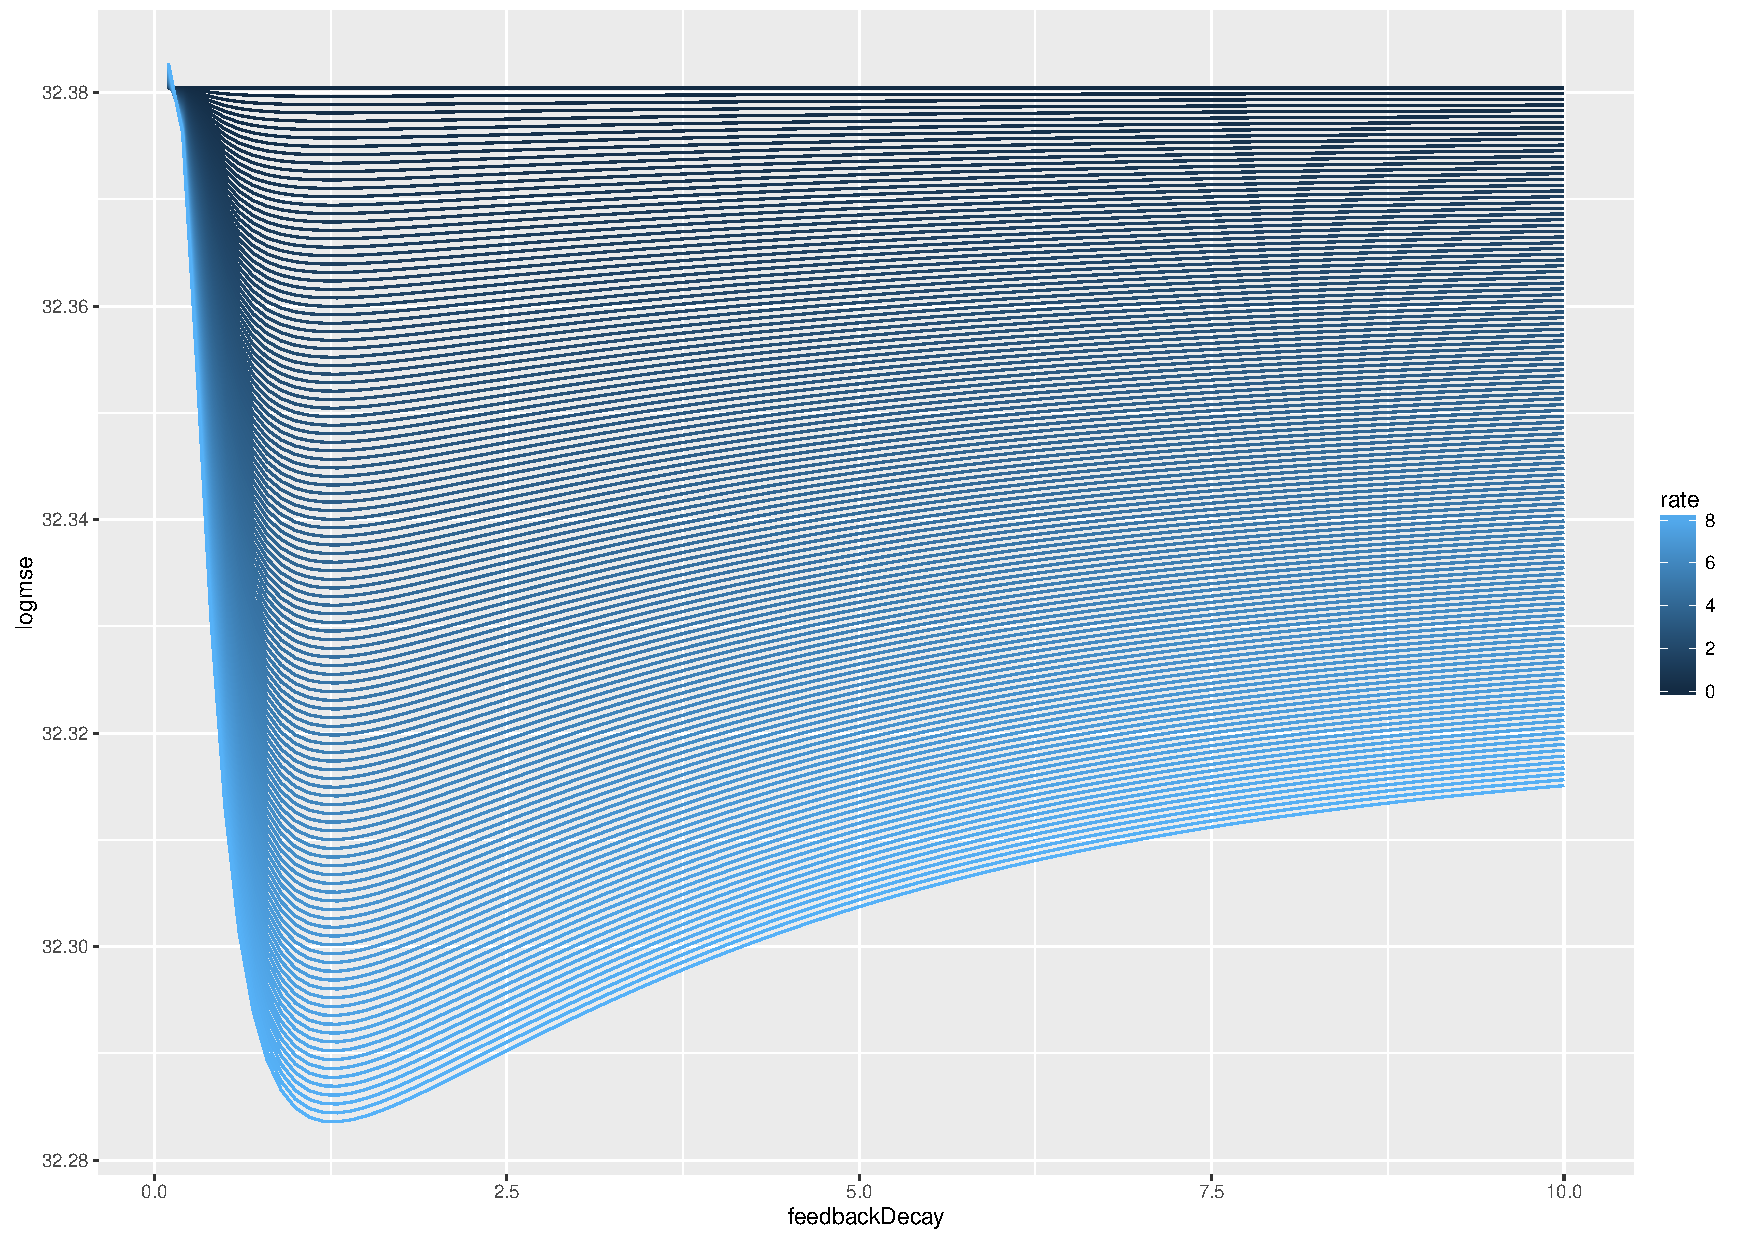
\includegraphics[width=0.55\textwidth]{figures/logmse-feedbackDecay_ZOOM}
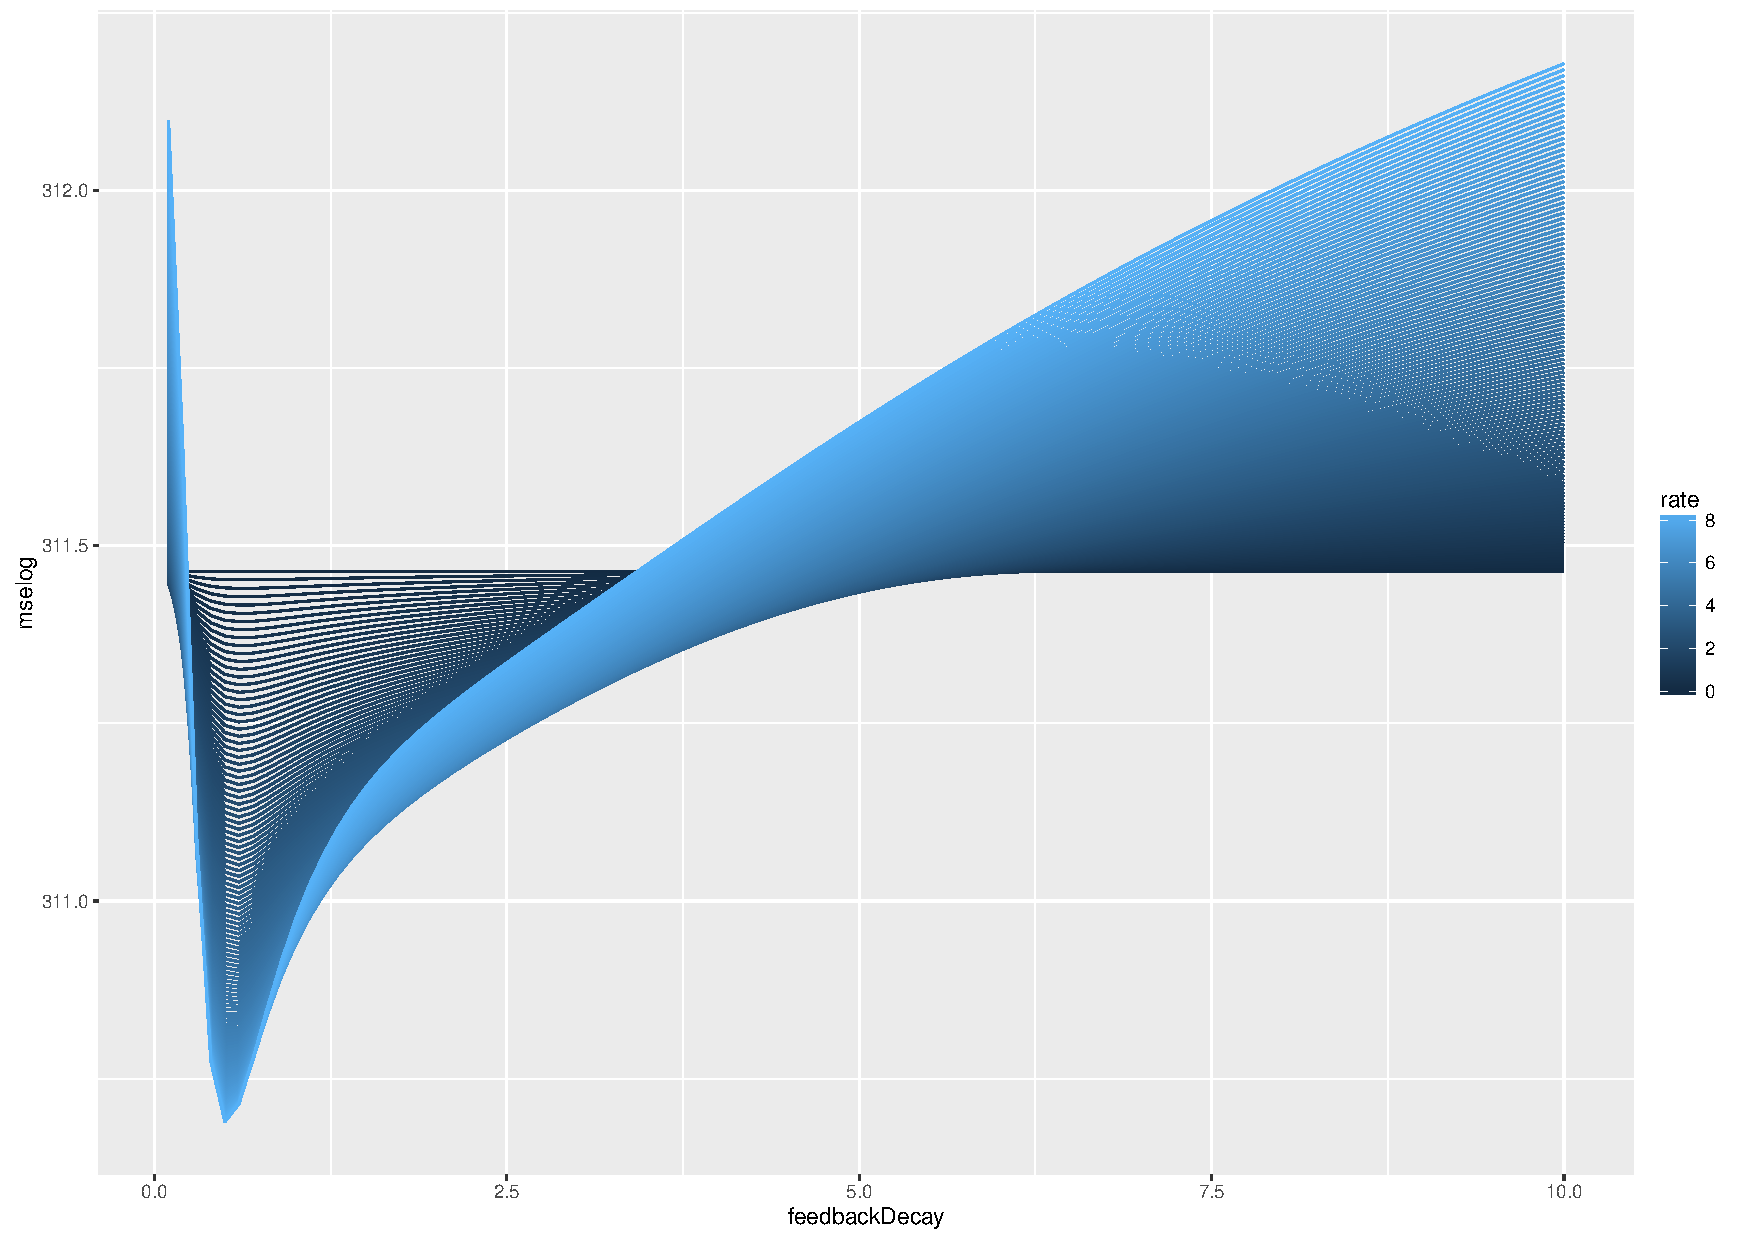
\includegraphics[width=0.55\textwidth]{figures/mselog-feedbackDecay_ZOOM}


}

\sframe{Exploration}{
\textit{Feedback with fixed gravity : first evidences of network effects ; confirmed with effect of $\alpha_0$}

\medskip

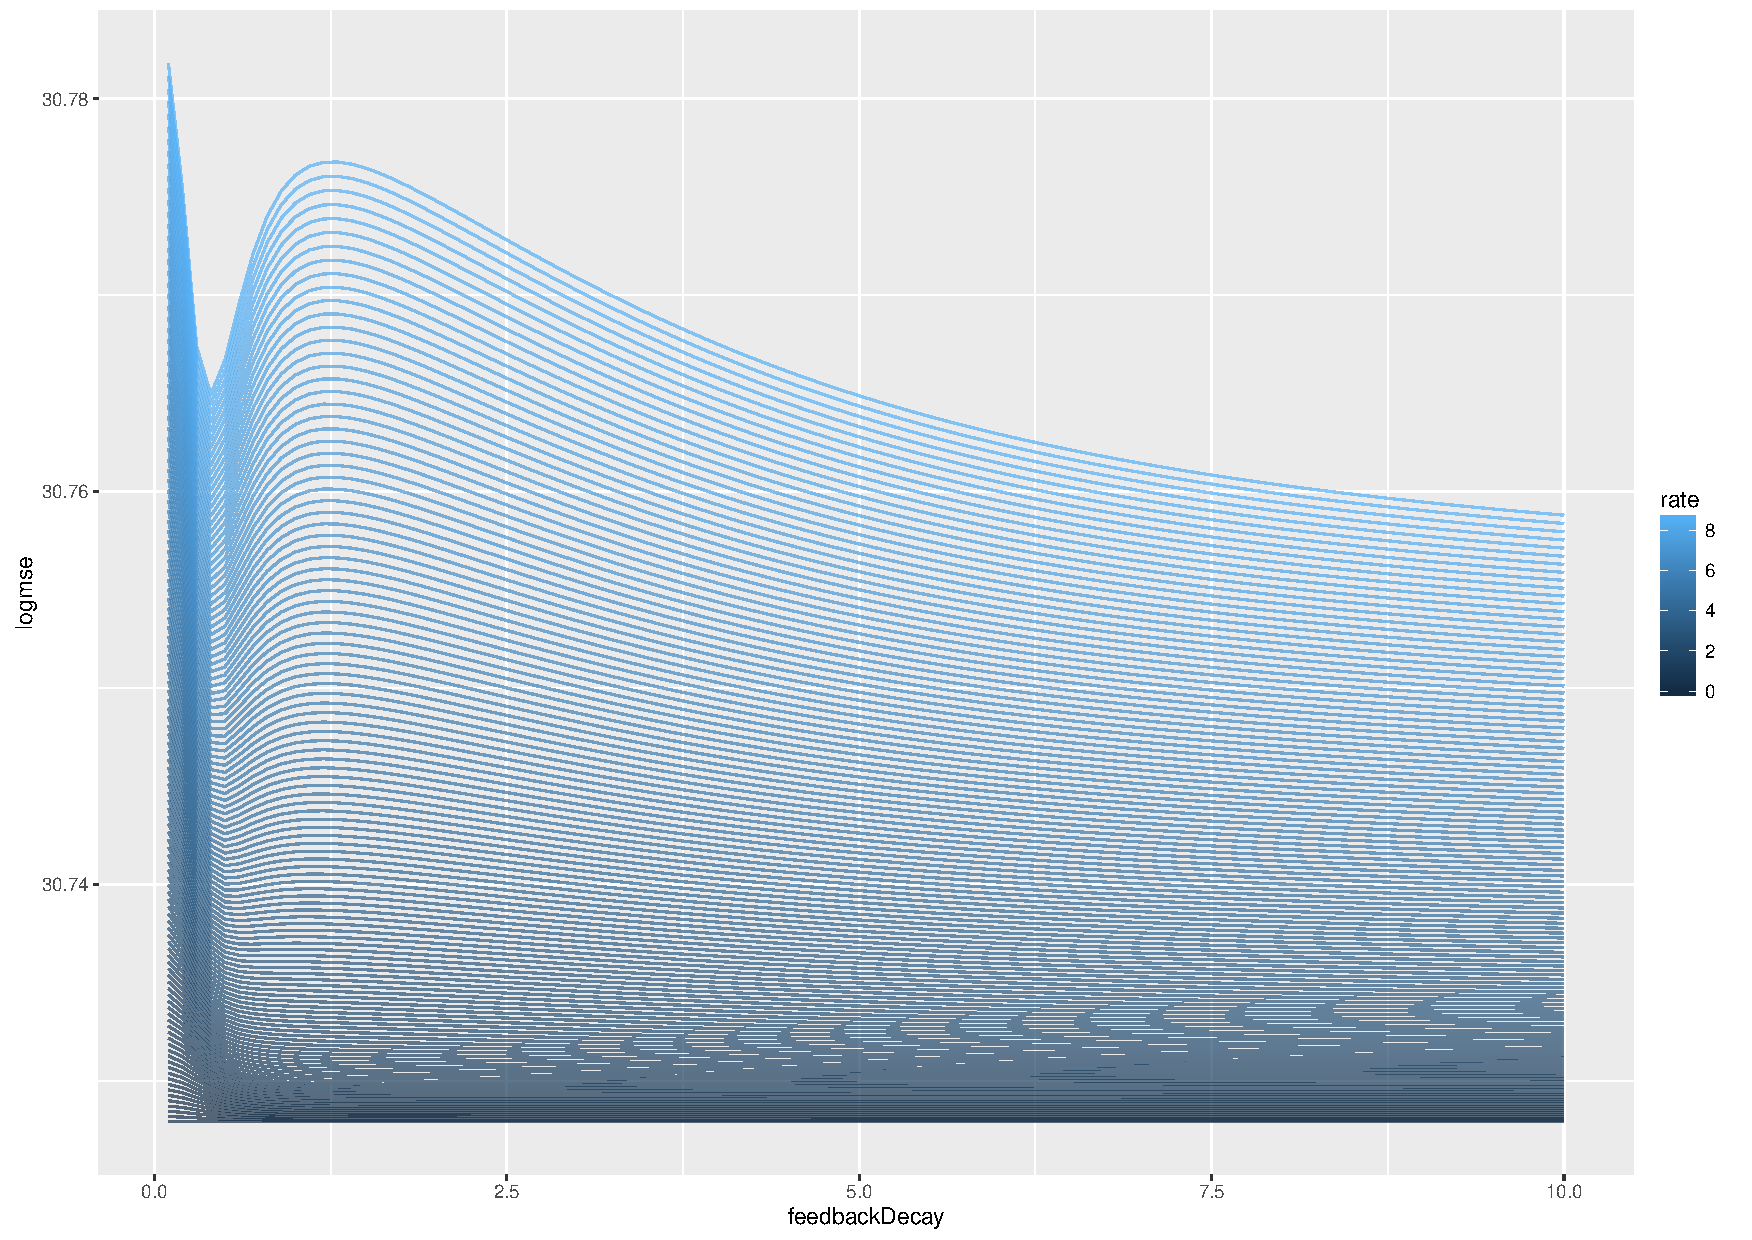
\includegraphics[width=0.55\textwidth]{figures/logmse-feedbackDecay_ZOOM_fixedgravity}
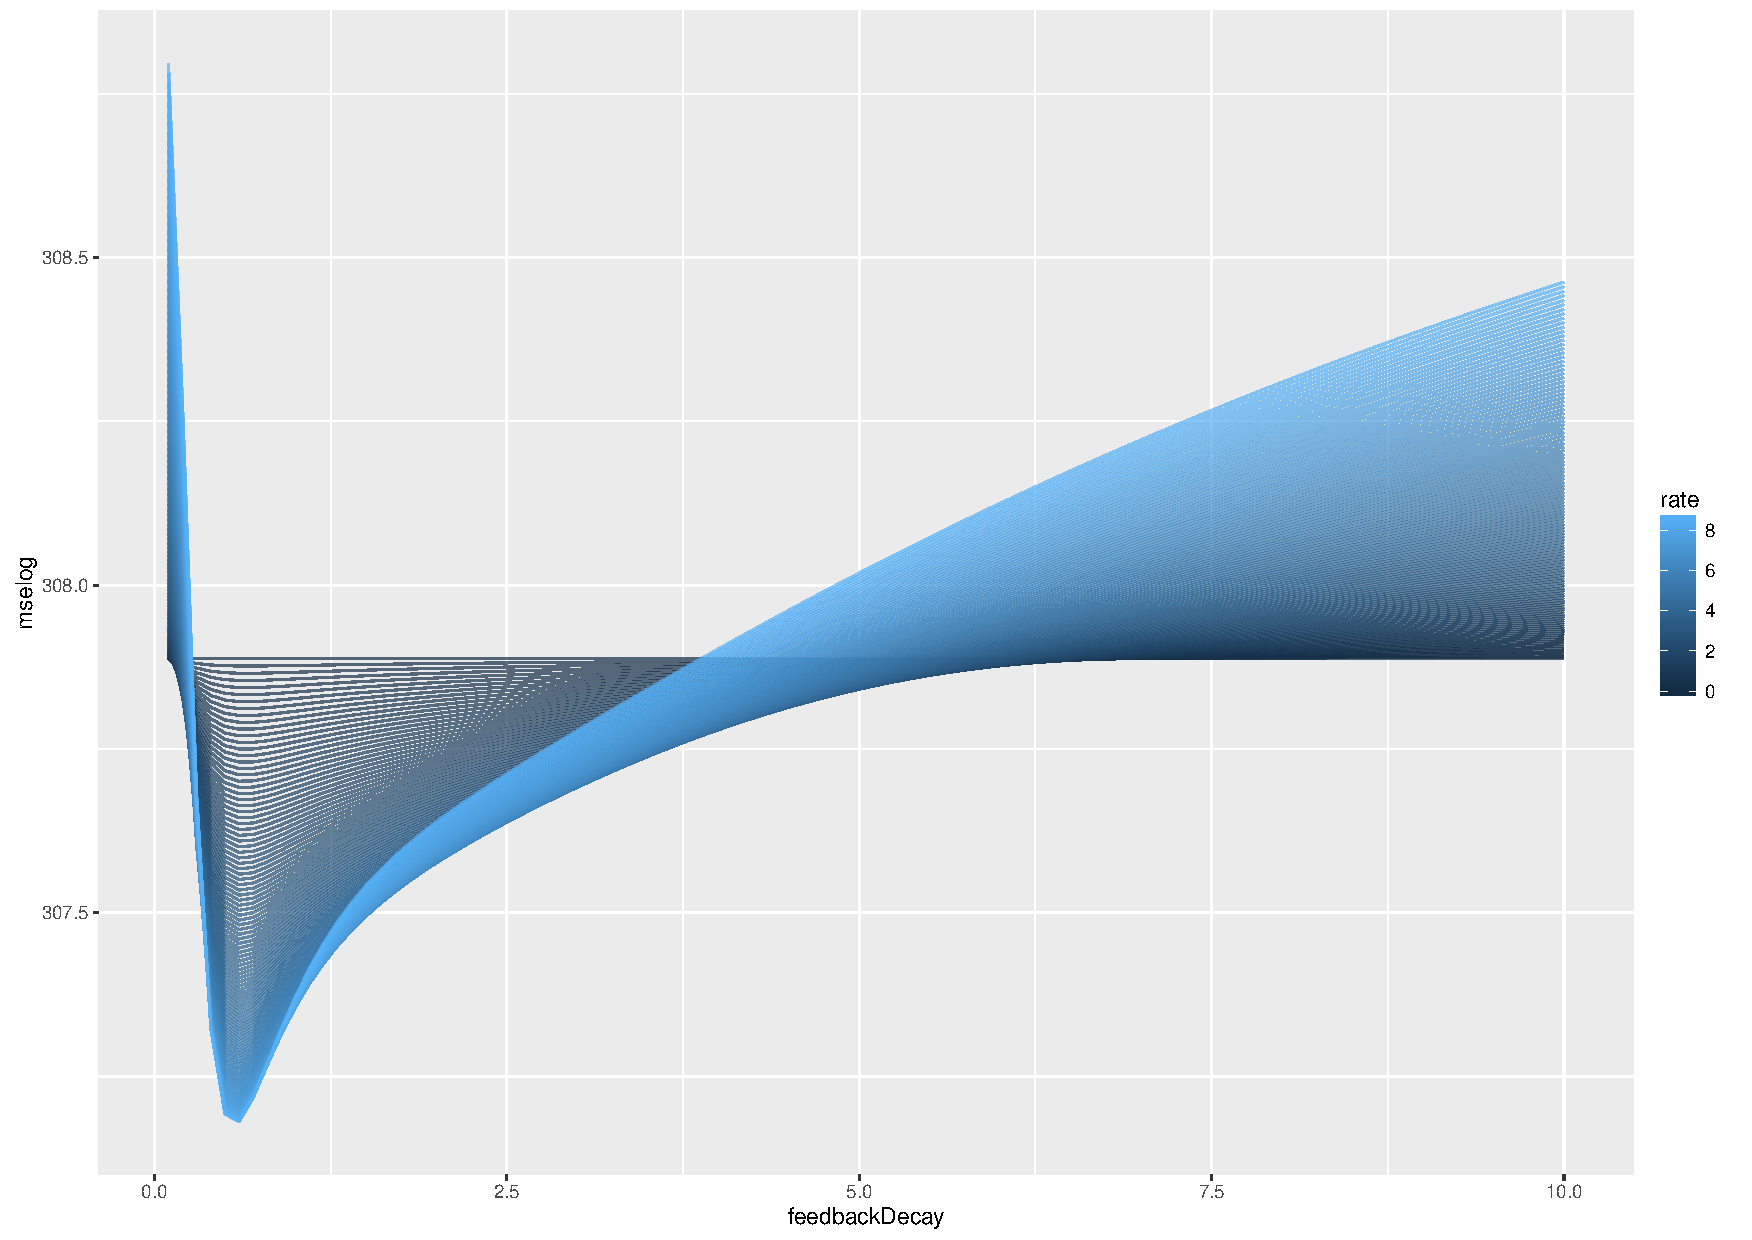
\includegraphics[width=0.55\textwidth]{figures/mselog-feedbackDecay_ZOOM_fixedgravity}


}


\sframe{Calibration}{
\textit{Gravity only}

% Pareto fronts

\medskip

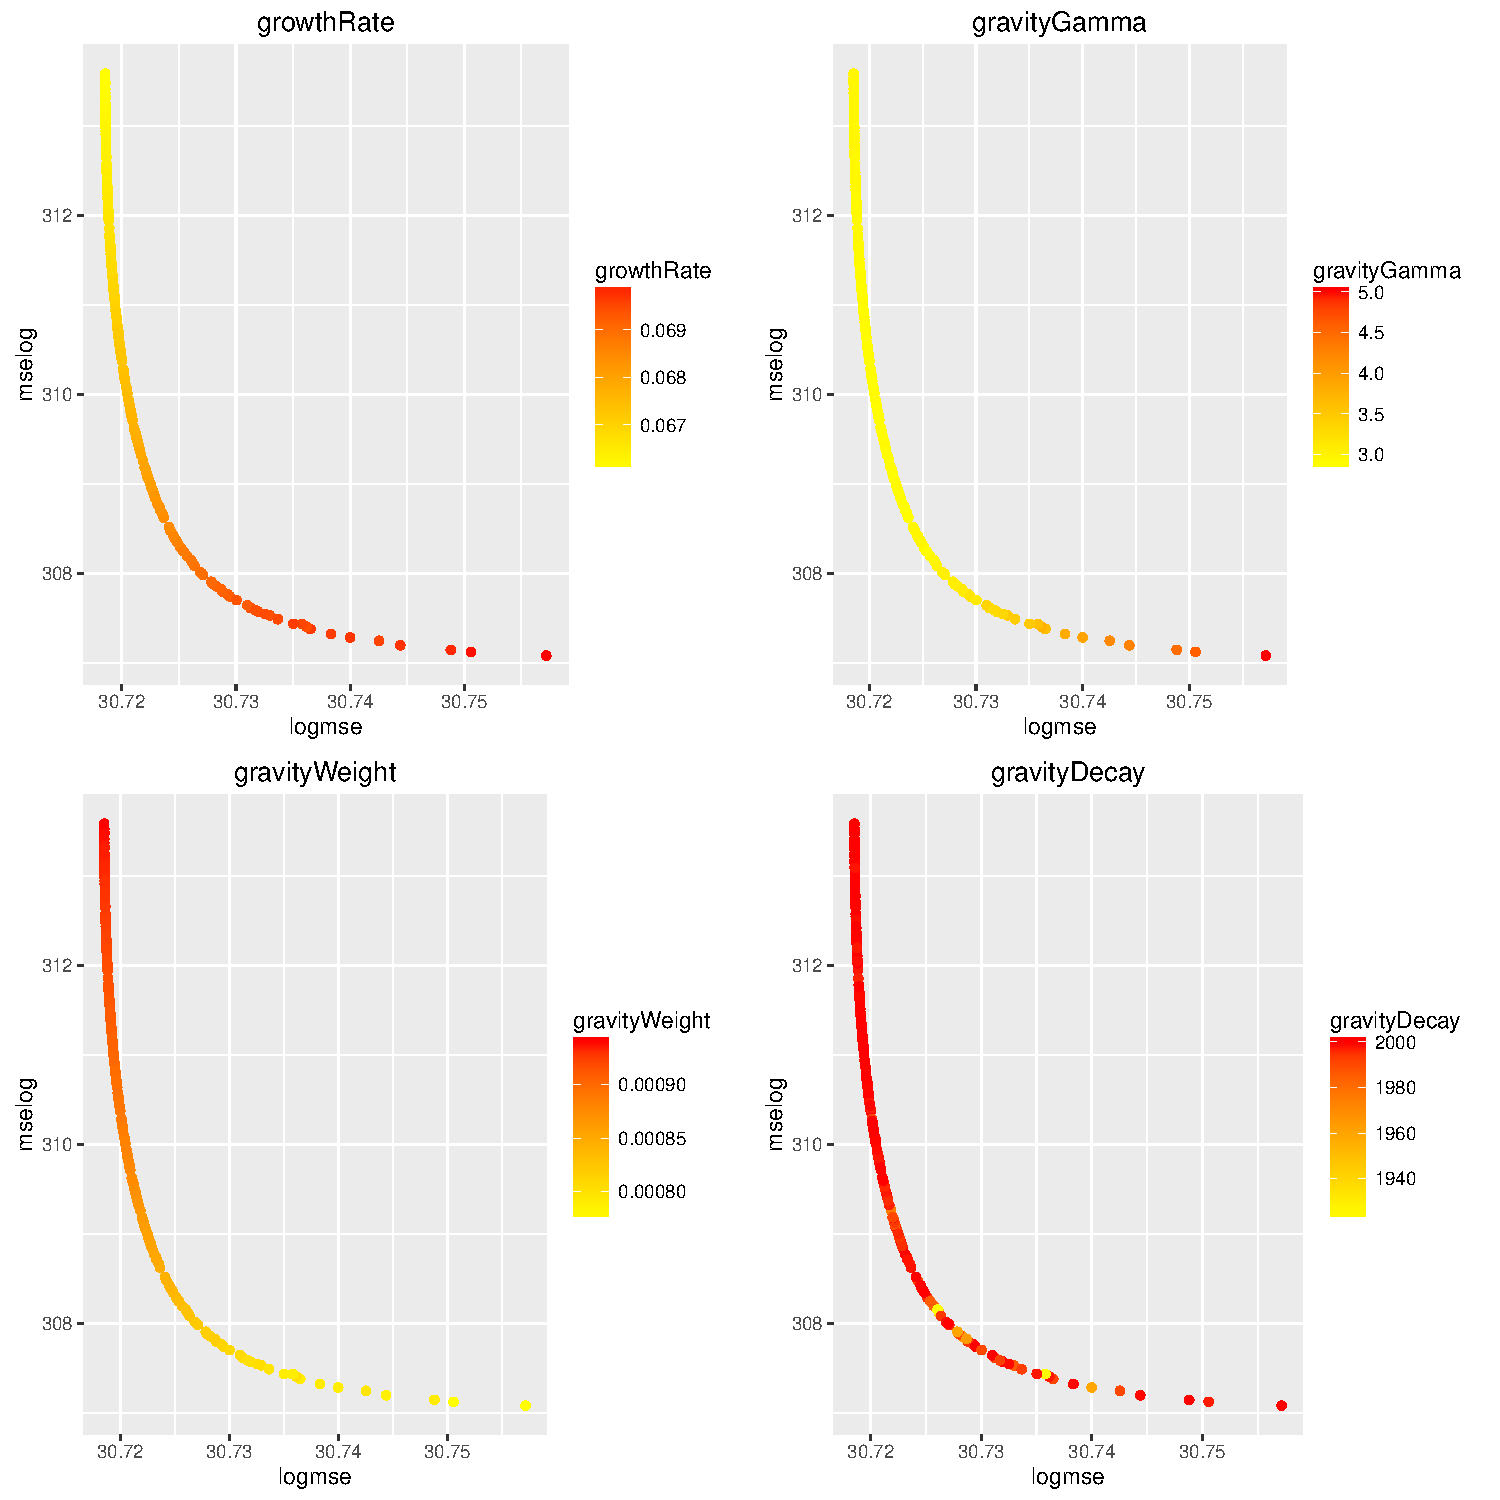
\includegraphics[height=0.8\textheight,width=0.9\textwidth]{figures/calib_nofeedback_pareto}

}

\sframe{Calibration}{
\textit{Feedback only}

\medskip
% Pareto

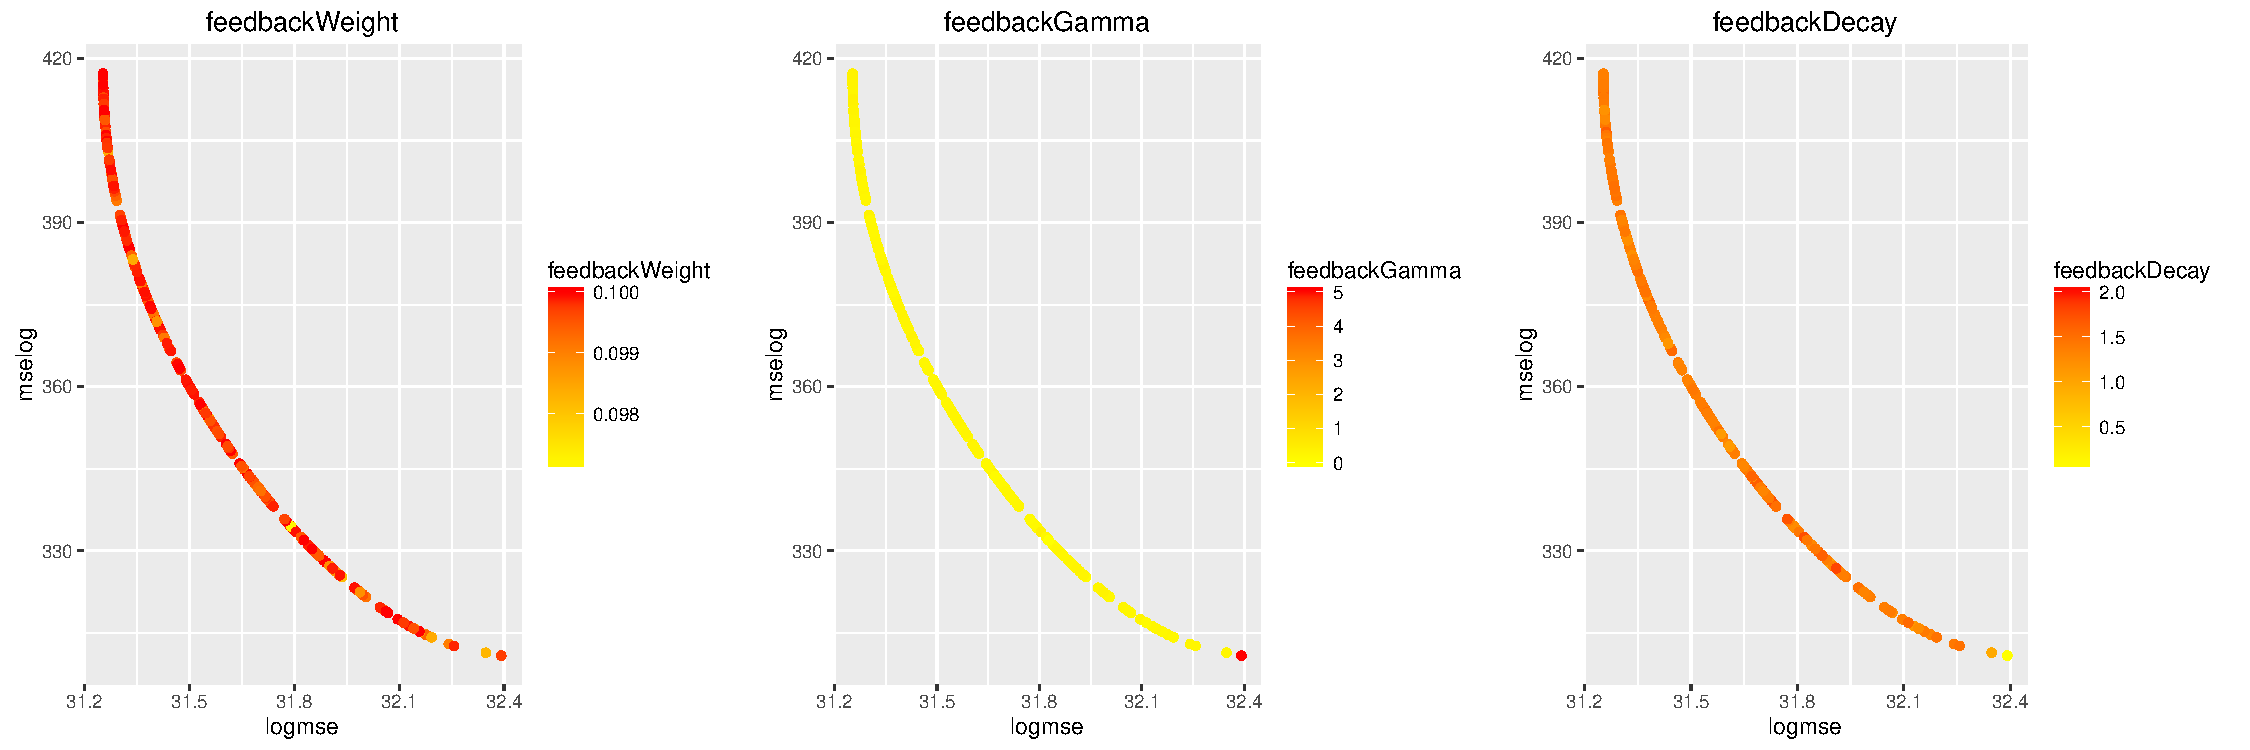
\includegraphics[width=1.1\textwidth]{figures/calib_nogravity_pareto}


}

\sframe{Calibration}{
\textit{Full Model, Iterative Calibration}

% fixed gravity Pareto Front

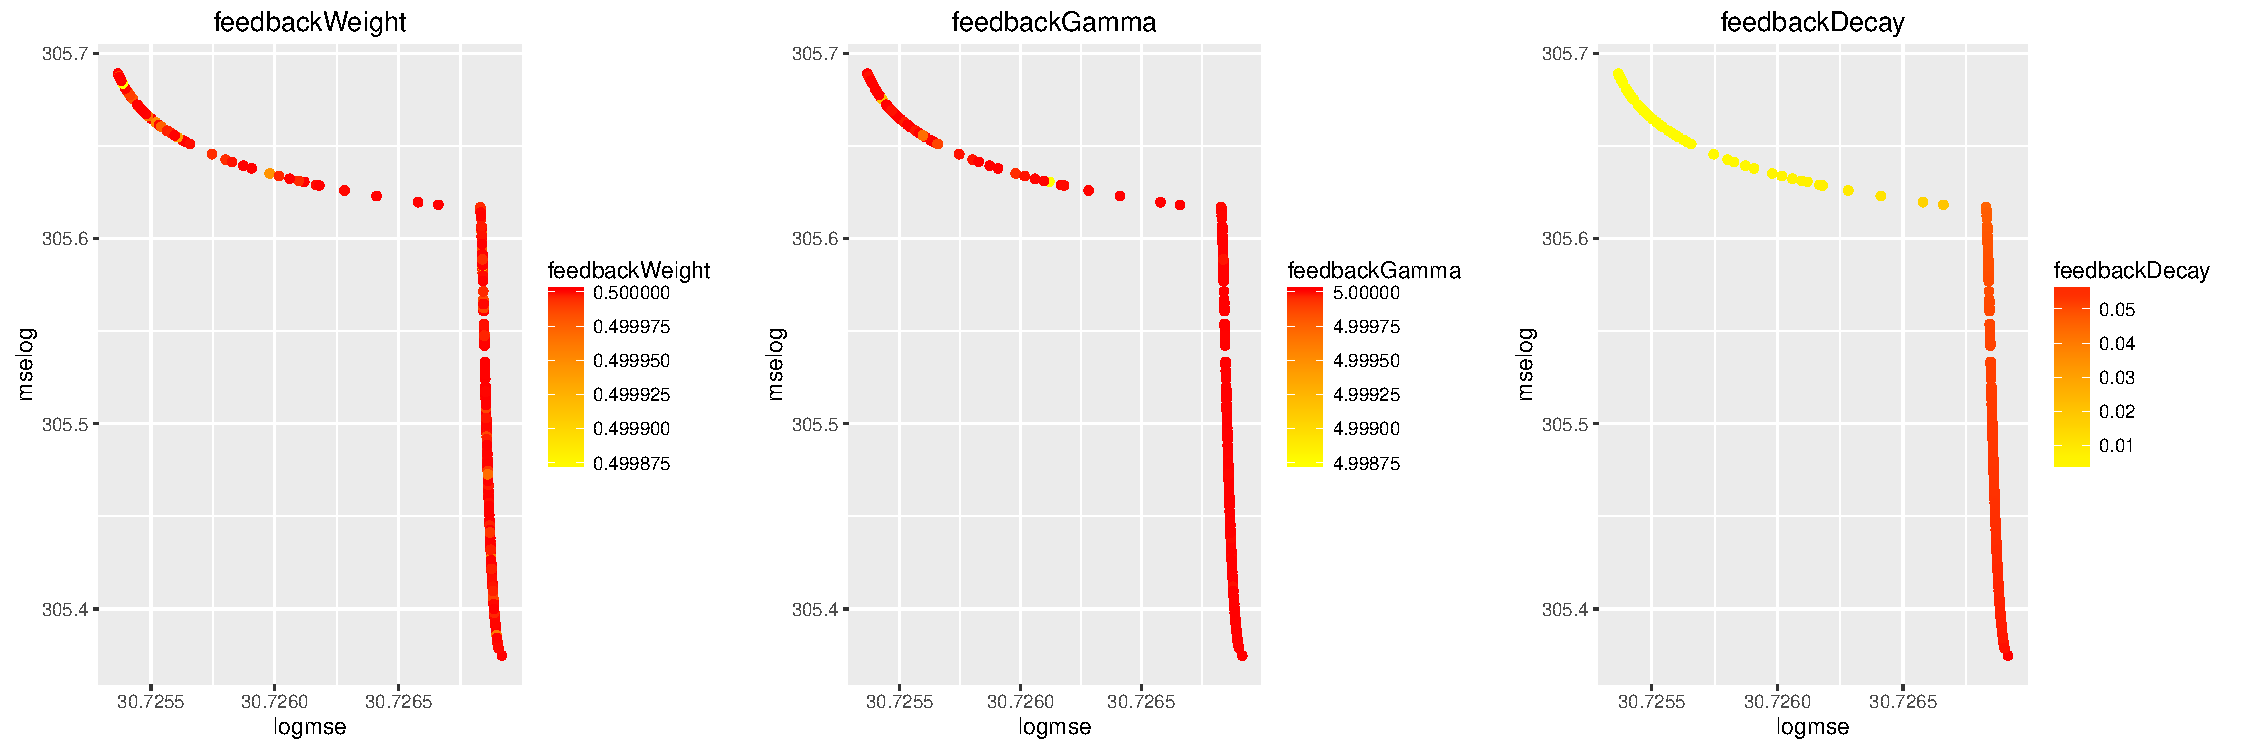
\includegraphics[width=\textwidth]{figures/calib_fixedgravity_pareto}

}

\sframe{Calibration}{
\textit{Full Model}

% full calib Pareto Front

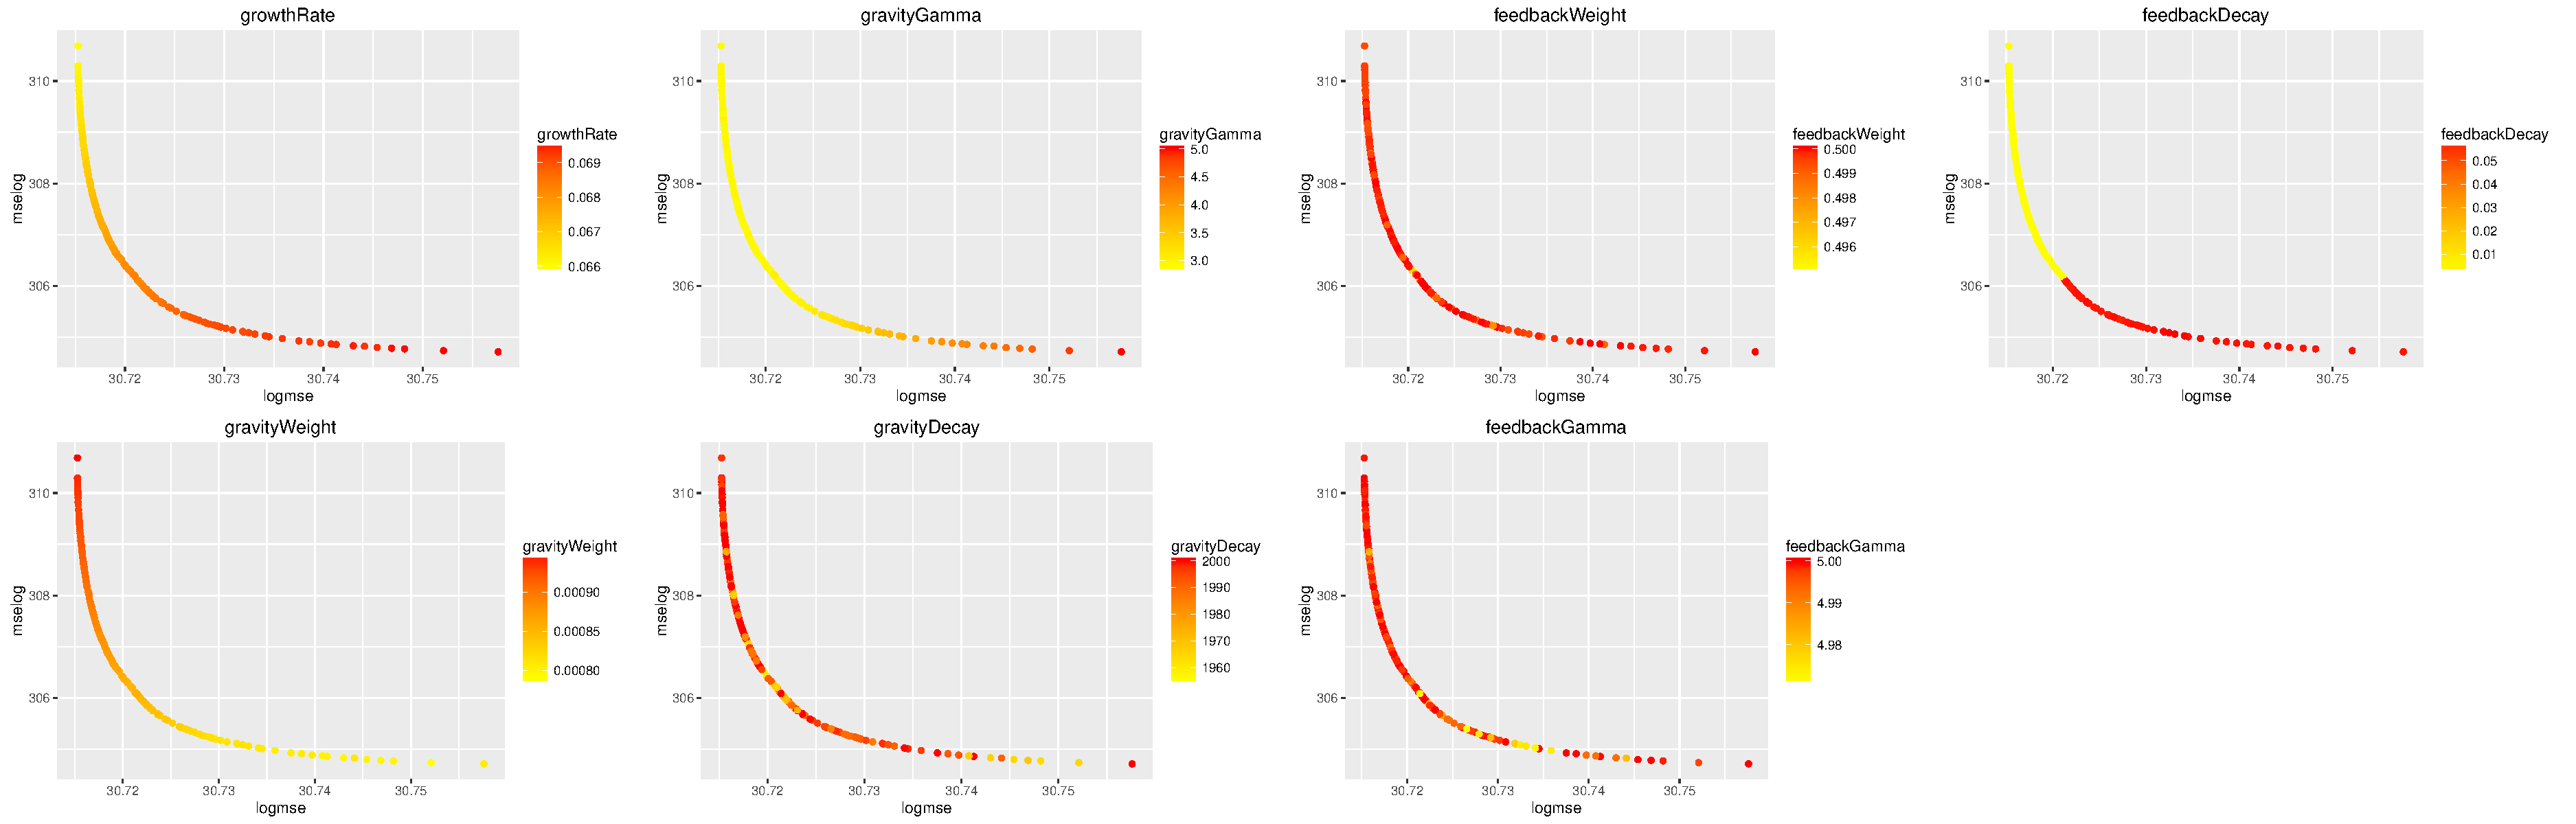
\includegraphics[width=1.1\textwidth,height=0.8\textheight]{figures/calib_fullmodel_pareto}

}
%
%\sframe{Profiles}{
%\textit{Full Model}
%
%% full calib Pareto Front
%
%}
%

\sframe{Temporal moving window}{
\textit{Calibration by normalized periods (no wars, same number of data points)}
%  gravity only calib

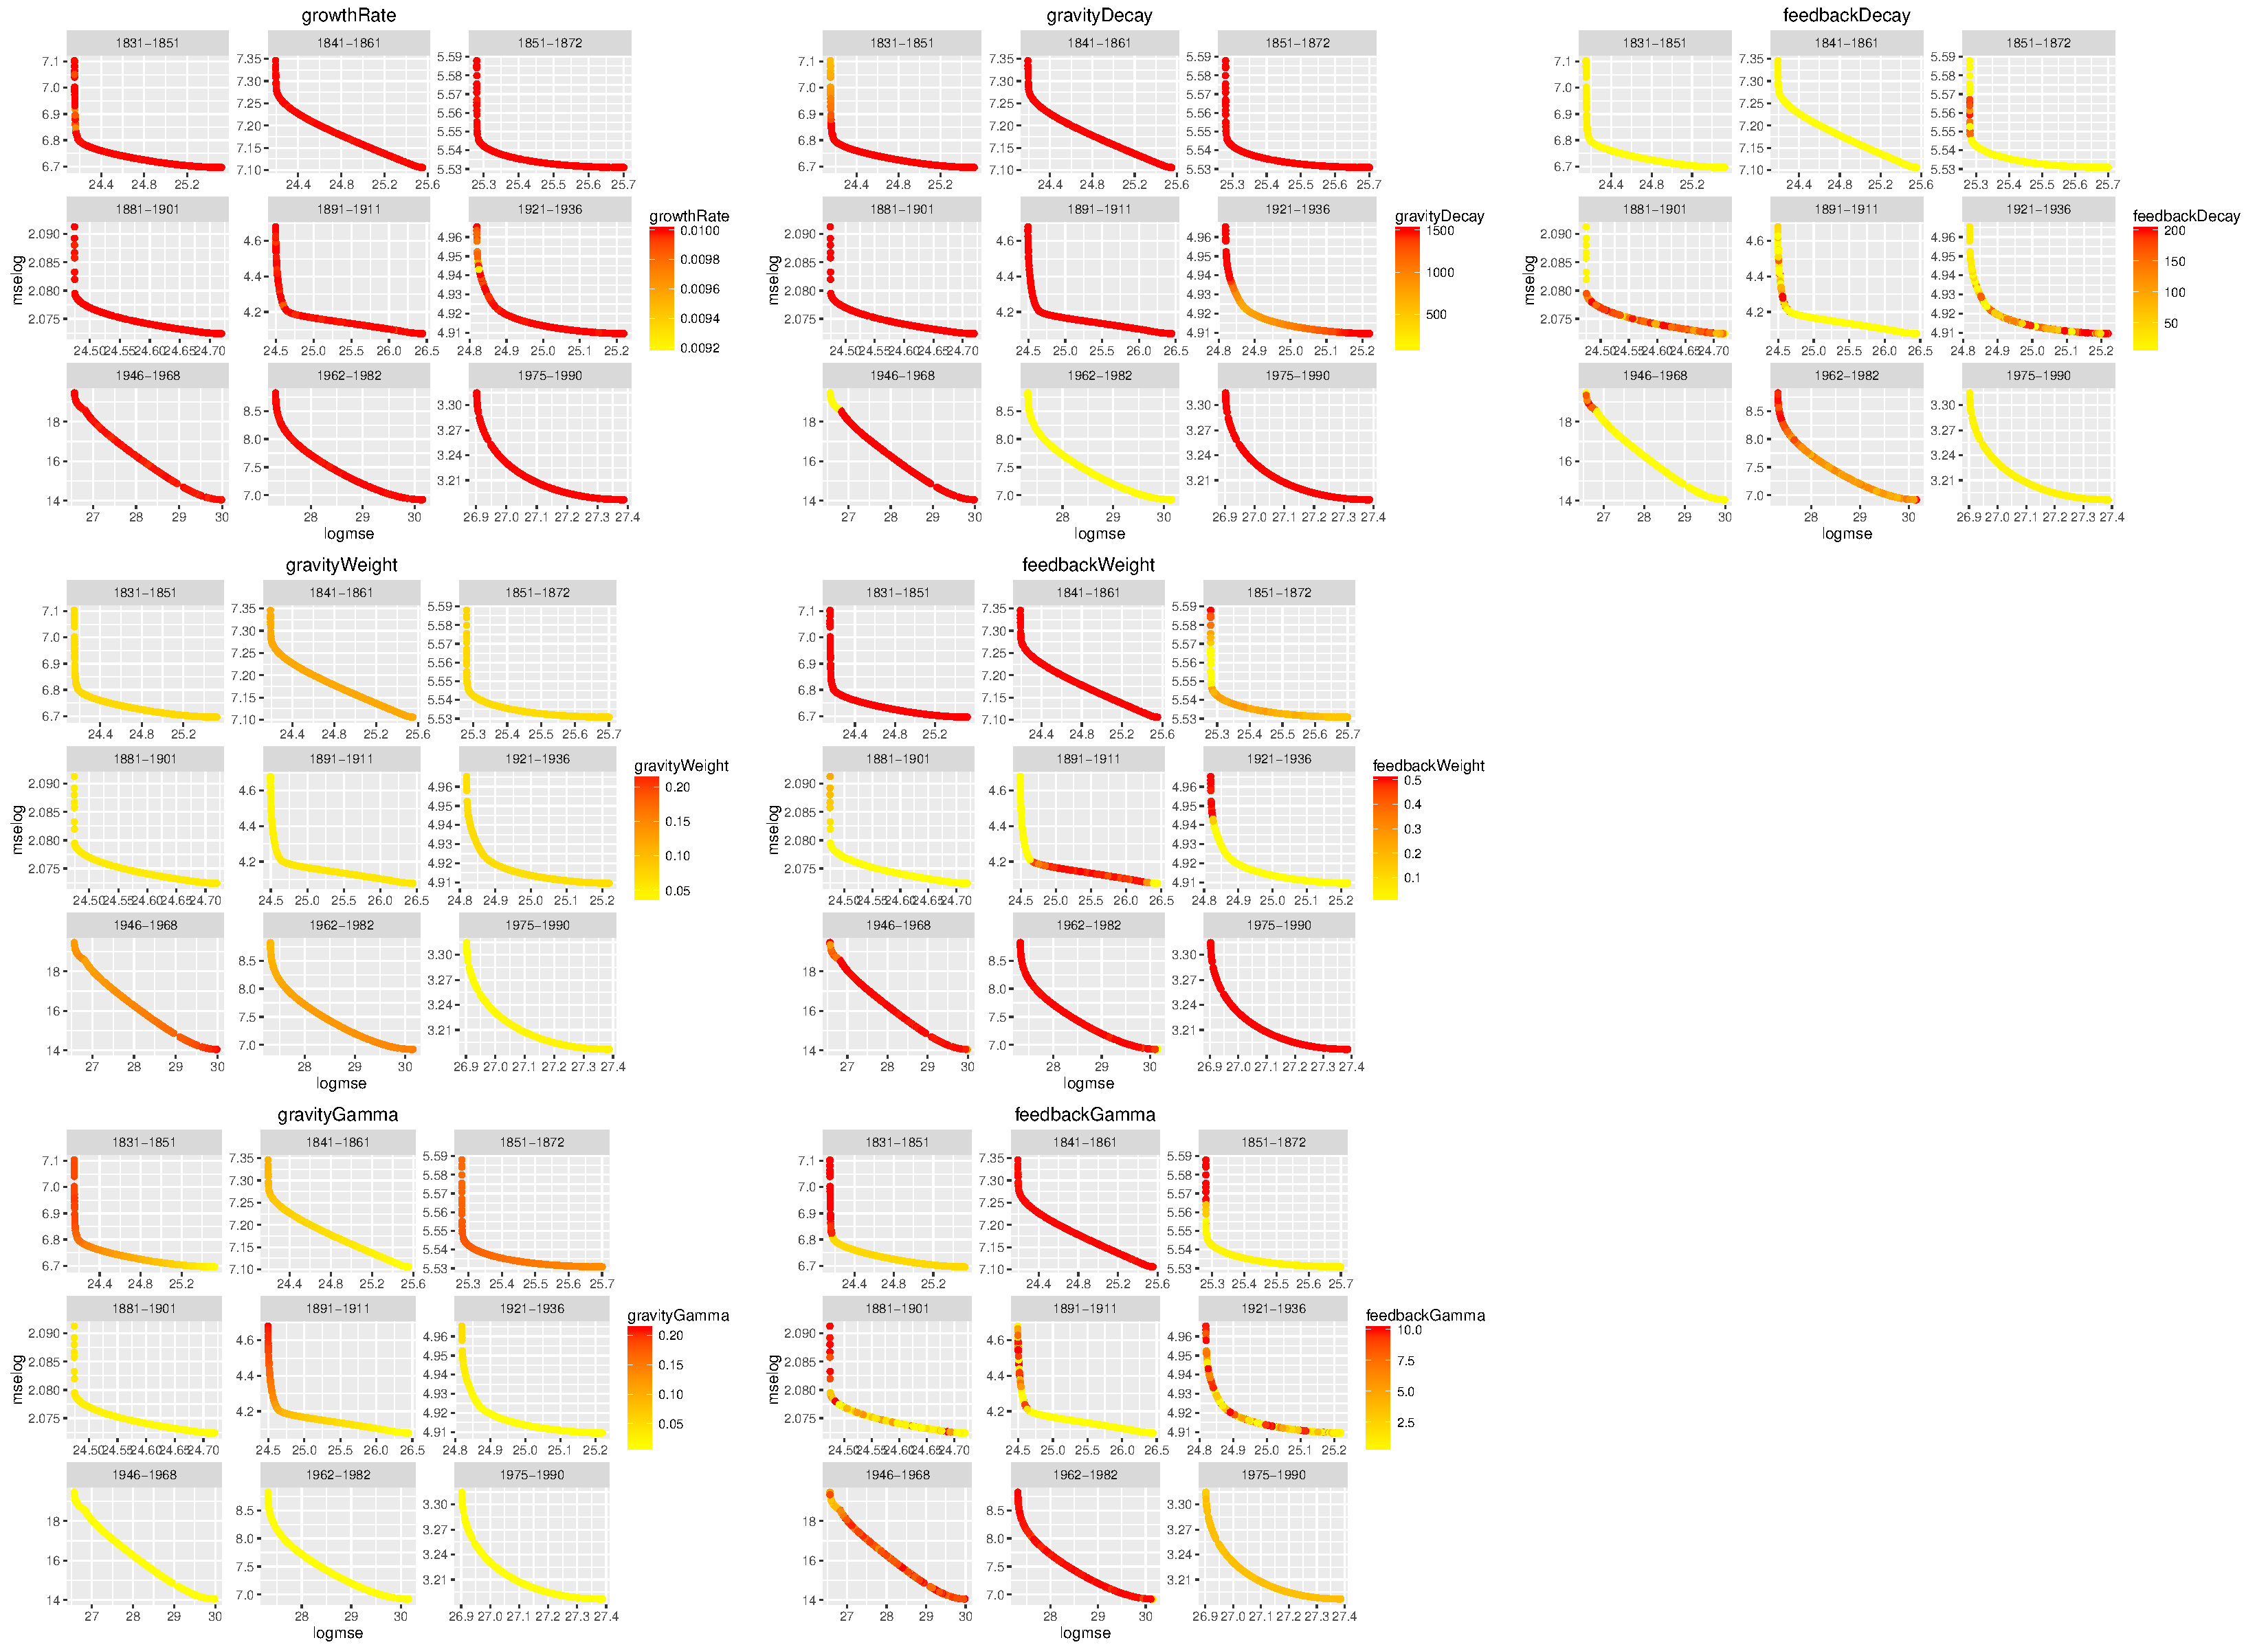
\includegraphics[width=1.1\textwidth,height=0.8\textheight]{figures/allperiods_allparams}


}

%\sframe{Temporal moving window}{
%% conditioned feedback by periods
%
%% full calib period ? -> not sure.
%
%}


\sframe{Next steps}{
\begin{itemize}
\item Compute empirical AIC to check if improvement is worth additional parameters. Various approaches :
\begin{itemize}
\item Via empirical likelihood
\item Via non-linear sparse regression
\item Via behavior space and statistical multimodeling
\end{itemize}
\item Calibration profiles (still running)
\item Link with models with covariance : propose a general framework (extending the Simon-Gibrat work)
\end{itemize}
}





%\sframe{Methodological Issue}{
%
%\textbf{Next step : } Introduce feedback terms due to effective physical flows passing through the city (in a first approximation only geographically computed with elevation data), test directly for network necessity. Fitting that model should also allow to quantify tunnel effect (strength of feedback).
%
%\bigskip
%
%\textbf{Methodological Flaw : } Issue with overfitting in models of simulations (seems to be an open question) : how do we know fit improvement is not only due to additional degree of freedom ? In stats : AIC provides Kullback-leibler information gain by correcting log-likelihood with number of parameters, nothing similar for models of simulation. Possible solutions :
%\small
%\begin{enumerate}
%\item Empirical version of AIC : Brutal version with empirical likelihood ? Estimation of statistical models on parameter space of each model of simulation, use of corresponding AIC ?
%\item Sparse non-linear machine learning to produce a kind of ``absolute'' benchmark explainable variance at a given number or parameters (rq : simple 2nd degree polynomial autoregressive model give far better results than two models above !)
%\end{enumerate}
%
%
%}
%







\section{Thesis Organisation}



\jframe{Spatial Statistics}{

\textit{First work on Granger causality for spatial statistics : synthetic data by RBD model}

\medskip

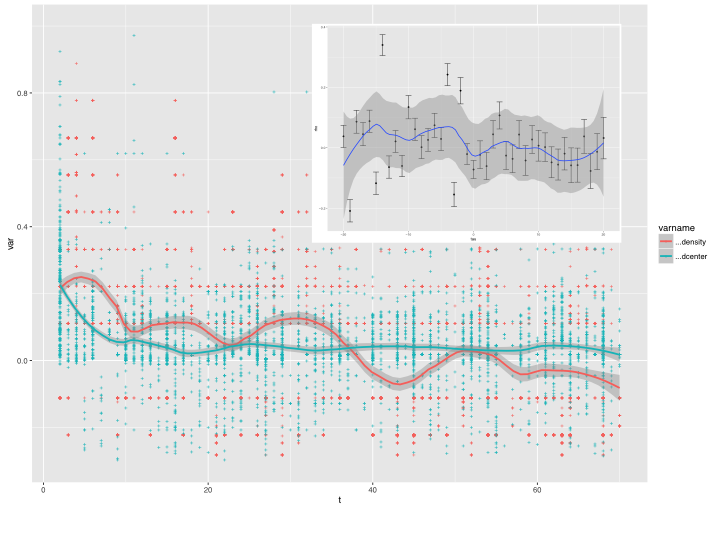
\includegraphics[width=0.8\textwidth]{figures/synth}

}



\jframe{Thesis Organisation}{
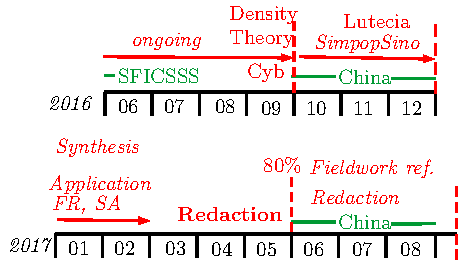
\includegraphics[width=\textwidth]{figures/edt}
}

%\jframe{Papers}{
%\begin{itemize}
%}



%%%%%%%%%%%%%%%%%%%%%%%%%%%%%%%%
\jframe{Next steps (until August 30th 2016)}{
\begin{itemize}
\item SFICSSS [4w] (+ holidays [2w])\medskip
\item Cybergeo Paper [1w]\medskip
\item Density Paper [1w]\medskip
\item Theoretical Paper [1w]\medskip
\item Static Correlations (presentation at RGS conference on 31th) [1w]\medskip
\item China project [1w]\medskip
\end{itemize}
}






%%%%%%%%%%%%%%%%%%%%%%%%%%%%%%%%
%\begin{frame}[allowframebreaks]
%\frametitle{References}
%\bibliographystyle{apalike}
%\bibliography{/Users/Juste/Documents/ComplexSystems/CityNetwork/Biblio/Bibtex/CityNetwork}
%\end{frame}
%%%%%%%%%%%%%%%%%%%%%%%%%%%%%%%%


\end{document}




